\documentclass[
12pt,
a4paper,
% pointednumbers,        % überschriftnummerierung mit Punkt 
pointlessnumbers ,      % überschriftnummerierung ohne Punkt 
]{scrartcl}
%% Optional Packages. 
%% Choose packages you want by using comments in the list below. 

\usepackage[
%% en, %% English text and wording
de, %% German text and wording
singlepage, %% Put sitenumbers always on the right
%%doublepage, %% Put sitenumbers alternating on the left and on the right. The first number starts always right, so be sure that you insert a blank page with \shipout\null
acronym, %% Use acronyms and print a acronym table. Use acronym.tex to add acronyms
figures, %% make list of figures and include graphicx package
tables, %% make list of tables and include table packages, also supertabular
listings, %% Use listings for source code and create table of listings
%% intro, %% include introduction file and make bookmark
 bib, %% make list of references at the end and import bib package. Use bib.bib as bibliography
%% appendix, %% includes appendix. add sections in the file appendix.tex
%% PA, %% inserts at the titlepage the company and such stuff
%% Bachelor, %% inserts at the titlepage the company and such stuff: Bachelorformat
Study, %% insert at the titlepage information without company and such stuff
%% 2010, %% Bis Jahrgang 2010 --> Ehrenwörtliche Erklärung
2011, %% Ab Jahrgang 2011 --> Ehrenwörtliche Erklärung
]{optional} 
 
\opt{en}{\usepackage[american]{babel}} 
\opt{de}{\usepackage[ngerman]{babel}}

% %%% Folgende Angaben ausfüllen:

\newcommand{\student}{Marco Heumann} 
\newcommand{\matrikel}{4188528}  
\newcommand{\kurs}{TINF13AI-BI}  

\newcommand{\reporttitle}{Programmierung einer SIM-Authentifizierung}  
\newcommand{\reportsubtitle}{Irgend ein Untertitel}

\opt{en}{\newcommand{\reportstart}{startdate}} 
\opt{de}{\newcommand{\reportstart}{startdatum}} 
\opt{en}{\newcommand{\reportend}{enddate}}
\opt{de}{\newcommand{\reportend}{enddatum}}
\opt{en}{\newcommand{\handoverdate}{}}
\opt{de}{\newcommand{\handoverdate}{}}
\opt{en}{\newcommand{\timerange}{}}
\opt{de}{\newcommand{\timerange}{}}

\newcommand{\tutor}{}
\newcommand{\companylogo}{dblogo} %% filname of logo for titlepage
\opt{Study}{
	\newcommand{\reportsemester}{5. - 6. Semester}
}
\opt{PA}{
	\newcommand{\businessunit}{I.LPA 73} 
	\newcommand{\department}{}
	\newcommand{\company}{DB Systel GmbH}
	\opt{en}{\newcommand{\educationdepartment}{Education department}}
	\opt{de}{\newcommand{\educationdepartment}{Fakult{\"a}t f{\"u}r Technik}}
	\opt{en}{\newcommand{\lokation}{Frankfurt}}
	\opt{de}{\newcommand{\lokation}{Frankfurt a. Main}}
	\newcommand{\manager}{Detlef Exner}
}
\opt{Bachelor}{
	\newcommand{\degree}{Bachelor of Science}
	\newcommand{\company}{Company}
	\newcommand{\lokation}{Mannheim}
}


\newcommand{\dhbws}{DHBW Mannheim}
\opt{en}{\newcommand{\dhbw}{BW Cooperative State University Mannheim, Germany}}
\opt{de}{\newcommand{\dhbw}{Duale Hochschule Baden-W{\"u}rttemberg Mannheim}}
\opt{en}{\newcommand{\studiengang}{applied computer science}}
\opt{de}{\newcommand{\studiengang}{Angewandte Informatik}}
\newcommand{\prof}{Prof. Dr. C. B{\"u}rgy} % Tutor at DHBW

\opt{listings}{
	\newcommand{\listingssetup}{
		\lstset{
			language={[Visual]Basic},                  % the language of the code
			basicstyle=\footnotesize,       % the size of the fonts that are used for the code
			numbers=left,                   % where to put the line-numbers
			numberstyle=\tiny\color{gray},  % the style that is used for the line-numbers
			stepnumber=0,                   % the step between two line-numbers. If it's 1, each line 
			                                % will be numbered
			numbersep=5pt,                  % how far the line-numbers are from the code
			backgroundcolor=\color{white},  % choose the background color. You must add \usepackage{color}
			showspaces=false,               % show spaces adding particular underscores
			showstringspaces=false,         % underline spaces within strings
			showtabs=false,                 % show tabs within strings adding particular underscores
			frame=single,                   % adds a frame around the code
			rulecolor=\color{black},        % if not set, the frame-color may be changed on line-breaks within not-black text (e.g. commens (green here))
			tabsize=2,                      % sets default tabsize to 2 spaces
			captionpos=b,                   % sets the caption-position to bottom
			breaklines=true,                % sets automatic line breaking
			breakatwhitespace=false,        % sets if automatic breaks should only happen at whitespace
			title=\lstname,                 % show the filename of files included with \lstinputlisting;
			                                % also try caption instead of title
			keywordstyle=\color{blue},      % keyword style
			commentstyle=\color{green},   % comment style
			stringstyle=\color{gray},       % string literal style
			escapeinside={\%*}{*)},         % if you want to add LaTeX within your code
			morekeywords={*,...}            % if you want to add more keywords to the set
		}
	}
}

%%%%%%%%%%%%
%% Folgende Angaben müssen nicht verändert werden. Werden aber zur einfacheren Anpassung (falls nötig) hier aufgeführt
\opt{PA}{
	\opt{en}{\newcommand{\reporttype}{Internship Report}}
	\opt{de}{\newcommand{\reporttype}{Projektarbeit}}
}
\opt{Bachelor}{
	\opt{en}{\newcommand{\reporttype}{Bachelor thesis}}
	\opt{de}{\newcommand{\reporttype}{Bachelorarbeit}}
}
\opt{Study}{
	\opt{en}{\newcommand{\reporttype}{Study Report}}
	\opt{de}{\newcommand{\reporttype}{Studienarbeit}}
}


\usepackage{lipsum}
\usepackage{fancyhdr} %für Kopf- und Fußzeilen
%\usepackage{scrpage2}
\usepackage[utf8]{inputenc} %Zeichenkodierung
\usepackage{caption}
\usepackage[]{units}
\usepackage{calc}
\usepackage{xcolor}
\usepackage{setspace}
\usepackage{pdfpages}
\usepackage{enumerate}
\usepackage{scrhack}
\usepackage{tabularx}
\usepackage{pifont}
\usepackage[pdftex,pdfborder={0 0 0}, bookmarksopenlevel=1,
bookmarksdepth=3]{hyperref} %Kreiert Links von der Table of Content zu Kapiteln (ohne optische Hervorhebung)

\opt{acronym}{\usepackage[footnote]{acronym}}
\opt{figures}{\usepackage{graphicx}}
\opt{tables}{
	\usepackage{hhline} %% extended line features for tables with \hhline{}
	\usepackage{multirow} %% merges several cells over rows: \multirow{Zeilen}{Breite}{Inhalt}; over columns: \multicolumn{Spalten}{Ausrichtung}{Inhalt}
	\usepackage{colortbl} %% use defined colors in tables
	\usepackage{booktabs} %% better horizontal lines in tables with \toprule[<breite>], \midrule[<breite>], \cmidrule[<breite>](trim){a-b}, \bottomrule 
	\usepackage{supertabular}
	\usepackage{longtable}
} 
\opt{listings}{
	\usepackage{listings} 
	\listingssetup
}

\hypersetup{
	pdftitle={\reporttype\ - \reporttitle},
	pdfauthor={\studentS, \studentH},
	pdfsubject={\reporttitle},
	pdfkeywords={\reporttype, \dhbws\opt{PA}{, \company}}
} 

\newcommand{\settocdepth}[1]{
	\addtocontents{toc}{
		\protect
		\setcounter{tocdepth}{#1}
	}
}

\newcommand{\head}[1] {
 	\lhead{\ifthispageodd{}{#1}}
 	\rhead{\ifthispageodd{#1}{}}
 }

\newcommand{\headAndToc}[1] {
	\head{#1}
	\addcontentsline{toc}{section}{#1}
}

\newcommand{\headAndTocENDE}[2] {
	\opt{en}{
		\headAndToc{#1}
	}
	\opt{de}{
		\headAndToc{#2}
	}
}

\newcommand{\uml}[1]{\textsf{#1}}

%% math
\usepackage{amsmath,amssymb,amsfonts}
\newcommand{\Z}{\mathbb{Z}}
\newcommand{\order}{\mathrm{order\:}}
\newcommand{\IV}{\mathrm{IV}}
\newcommand{\tmod}{\!\!\mod}



 \renewcommand\sectionmark[1]{%
  \def\sectionname{#1}%
  \markright{\thesection #1}%oder was aus immer 
  } 
  
  \renewcommand\subsectionmark[1]{%
  \def\subsectionname{#1}% 
  \markright{\thesubsection #1}%oder was aus immer 
  } 
	
\graphicspath{{./ref/images/}}
\newcommand*\lstinputpath[1]{\lstset{inputpath=#1}}
\lstinputpath{./ref/listings/}

\newlength{\iconwidth}
\setlength{\iconwidth}{1cm}
\definecolor{boxheadcol}{gray}{.6}
\definecolor{boxcol}{gray}{.9}
\newenvironment{displaybox}[2]{%
  \begin{center}
    \setlength\arrayrulewidth{0.75pt}%
    \arrayrulecolor{white}%
    \renewcommand{\arraystretch}{1.3}%
    \begin{tabular}{p{\iconwidth}p{\linewidth-4\tabcolsep-\iconwidth}}
      \multirow{2}{*}{#2}&\cellcolor{boxheadcol}\textbf{\sffamily\color{white}#1} \\%
      \hhline{~-}%
      &\cellcolor{boxcol}%
}{%
      \\
    \end{tabular}
    \arrayrulecolor{black}%
  \end{center}%
}

\newenvironment{Tip}{%
\begin{displaybox}{Information}{
\includegraphics[width=\iconwidth]{icon-tipp}}}%
{\end{displaybox}}

\newenvironment{Hint}{%
\begin{displaybox}{Hinweis}{
\includegraphics[width=\iconwidth]{icon-hinweis}}}%
{\end{displaybox}}


\newenvironment{xlist}[1]{%
  \begin{list}{}{%
    \settowidth{\labelwidth}{#1:}
    \setlength{\labelsep}{0.5cm}
    \setlength{\leftmargin}{\labelwidth}
    \addtolength{\leftmargin}{\labelsep}
    \setlength{\rightmargin}{0pt}
    \setlength{\parsep}{0.5ex plus 0.2ex minus 0.1ex}
    \setlength{\itemsep}{0 ex plus 0.2ex}
    \renewcommand{\makelabel}[1]{##1:\hfil}
    }
  }
{\end{list}}

% custom commands
\newcommand{\Abbildung}[1]{Abbildung~\ref{fig:#1}}
\newcommand{\Anhang}[1]{Anhang~\ref{#1}: \nameref{#1} auf S.~\pageref{#1}}
\newcommand{\Verweis}[1]{~\ref{#1}: \nameref{#1} auf S.~\pageref{#1}}

\title{\pebericht}
\author{\student}
\date{\handoverdate}

\begin{document}
\pagestyle{fancy}  
% \pagestyle{scrheadings}
% \automark[section]{chapter}
\fancyhfoffset{\marginparsep}
\renewcommand{\footrulewidth}{1.0pt}
\renewcommand{\headrulewidth}{1.0pt}
\renewcommand{\headheight}{30pt}

\setlength{\parindent}{0in}
\setlength{\parskip}{0.5em}
\clubpenalty 10000
\widowpenalty 10000

\chead{}
\cfoot{}
 
\opt{doublepage}{
	\lfoot{\ifthispageodd{}{\thepage}}	
	\rfoot{\ifthispageodd{\thepage}{}}
}
\opt{singlepage}{
	\lfoot{}	
	\rfoot{\thepage}
}

\pagenumbering{Roman}

\opt{en}{\pdfbookmark[1]{Titlepage}{titlepage}}
\opt{de}{\pdfbookmark[1]{Titelseite}{titlepage}}
\begin{titlepage} 
	\opt{PA}{
		\begin{center}

	\vspace{2.2cm}
	\opt{PA}{{\large \textbf{\educationdepartment}}\\}
	\vspace{0.1cm}
	{\large \textbf{\dhbw}}\\
	\vspace{2cm}
	
	\opt{PA} {
		\includegraphics*[width=4.5cm]{\companylogo} \quad\quad\quad\quad\quad \includegraphics*[width=4.5cm]{dhbwlogo}\\
	}
	\opt{Study}{
		\includegraphics*[width=7cm]{dhbwlogo}\\
	}
	
	\vspace{2.8cm}
	{\Large \textbf{\reporttype}}\\
	\vspace{1cm}
	\doublespacing
	{\Huge \textbf{\reporttitle}}\\ 
	\singlespacing 
	\vspace{1cm}
%	{\large \reportsubtitle}\\
	\vspace{6.8cm}
	\onehalfspacing
	  
	\opt{PA}{
		\opt{en}{
			\begin{tabbing}
				xxxxxxxxxxxxxx\=xxxxxxxxxxxxxxxxxxxxxxx\=xxxxxxxxxxxxx\=xxxxxxx\kill
				Name: \> {\textbf{\student}} \> Company: \> \company,\\
				{Matriculation}: \> \matrikel \> \> \educationdepartment\ \lokation\\
				Course: \> \kurs \> {Manager}: \> \manager\\
				Study course: \> \studiengang \> Department: \> \businessunit \\
				Study manager: \> \prof \> \> \department \\
				{Date:} \> \date{31/13/1331} \handoverdate \> {Tutor}: \> \tutor\\
			\end{tabbing}
		}
		   
		\opt{de}{
			\begin{tabbing}
				xxxxxxxxxxxxxxxx\=xxxxxxxxxxxxxxxxxxxxxxx\=xxxxxxxxxxxxx\=xxxxxxx\kill
				Name: \> {\textbf{\student}} \> Unternehmen: \> \company,\\
				{Matrikelnummer}: \> \matrikel \> \> \lokation\\
				Kurs: \> \kurs \> {Manager}: \> \manager\\
				Studiengang: \> \studiengang \> Abteilung: \> \businessunit \\
				Studiengangsleiter: \> \prof \> \> \department \\
				{Datum:} \> \date{31/13/1331} \handoverdate \> {Betreuer}: \> \tutor\\
			\end{tabbing}
		}
	}
	\opt{Study}{
		\opt{en}{
			\begin{tabbing}
				xxxxxxxxxxxxxx\=xxxxxxxxxxxxxxxxxxxxxxx\kill
				Name: \> {\textbf{\student}}  \\
				{Matriculation}: \> \matrikel  \\
				Course: \> \kurs \\
				Study course: \> \studiengang  \\
				Study manager: \> \prof  \\
				{Tutor}: \> \tutor  \\
				{Semester}: \> \reportsemester  \\
				{Date:} \> \date{31/13/1331} \handoverdate \\
				
			\end{tabbing}
		}
		   
		\opt{de}{
			\begin{tabbing}
				xxxxxxxxxx\=xxxxxxxxxxxxxxxxxxxxxxxxx\=xxxxxxxx\=xxxxxxxxx\kill
				Name: \> {\textbf{\studentS}} \> Name: \> {\textbf{\studentH}}\\
				Kurs: \> \kurs \> Kurs: \> \kurs \\
				Betreuer: \> \prof \\
			\end{tabbing}
		}
	}
	   \enlargethispage{\baselineskip}
	   \enlargethispage{\baselineskip}
	\singlespacing 

\end{center}  

	}
	\opt{Study}{
		\begin{center}

	\vspace{2.2cm}
	\opt{PA}{{\large \textbf{\educationdepartment}}\\}
	\vspace{0.1cm}
	{\large \textbf{\dhbw}}\\
	\vspace{2cm}
	
	\opt{PA} {
		\includegraphics*[width=4.5cm]{\companylogo} \quad\quad\quad\quad\quad \includegraphics*[width=4.5cm]{dhbwlogo}\\
	}
	\opt{Study}{
		\includegraphics*[width=7cm]{dhbwlogo}\\
	}
	
	\vspace{2.8cm}
	{\Large \textbf{\reporttype}}\\
	\vspace{1cm}
	\doublespacing
	{\Huge \textbf{\reporttitle}}\\ 
	\singlespacing 
	\vspace{1cm}
%	{\large \reportsubtitle}\\
	\vspace{6.8cm}
	\onehalfspacing
	  
	\opt{PA}{
		\opt{en}{
			\begin{tabbing}
				xxxxxxxxxxxxxx\=xxxxxxxxxxxxxxxxxxxxxxx\=xxxxxxxxxxxxx\=xxxxxxx\kill
				Name: \> {\textbf{\student}} \> Company: \> \company,\\
				{Matriculation}: \> \matrikel \> \> \educationdepartment\ \lokation\\
				Course: \> \kurs \> {Manager}: \> \manager\\
				Study course: \> \studiengang \> Department: \> \businessunit \\
				Study manager: \> \prof \> \> \department \\
				{Date:} \> \date{31/13/1331} \handoverdate \> {Tutor}: \> \tutor\\
			\end{tabbing}
		}
		   
		\opt{de}{
			\begin{tabbing}
				xxxxxxxxxxxxxxxx\=xxxxxxxxxxxxxxxxxxxxxxx\=xxxxxxxxxxxxx\=xxxxxxx\kill
				Name: \> {\textbf{\student}} \> Unternehmen: \> \company,\\
				{Matrikelnummer}: \> \matrikel \> \> \lokation\\
				Kurs: \> \kurs \> {Manager}: \> \manager\\
				Studiengang: \> \studiengang \> Abteilung: \> \businessunit \\
				Studiengangsleiter: \> \prof \> \> \department \\
				{Datum:} \> \date{31/13/1331} \handoverdate \> {Betreuer}: \> \tutor\\
			\end{tabbing}
		}
	}
	\opt{Study}{
		\opt{en}{
			\begin{tabbing}
				xxxxxxxxxxxxxx\=xxxxxxxxxxxxxxxxxxxxxxx\kill
				Name: \> {\textbf{\student}}  \\
				{Matriculation}: \> \matrikel  \\
				Course: \> \kurs \\
				Study course: \> \studiengang  \\
				Study manager: \> \prof  \\
				{Tutor}: \> \tutor  \\
				{Semester}: \> \reportsemester  \\
				{Date:} \> \date{31/13/1331} \handoverdate \\
				
			\end{tabbing}
		}
		   
		\opt{de}{
			\begin{tabbing}
				xxxxxxxxxx\=xxxxxxxxxxxxxxxxxxxxxxxxx\=xxxxxxxx\=xxxxxxxxx\kill
				Name: \> {\textbf{\studentS}} \> Name: \> {\textbf{\studentH}}\\
				Kurs: \> \kurs \> Kurs: \> \kurs \\
				Betreuer: \> \prof \\
			\end{tabbing}
		}
	}
	   \enlargethispage{\baselineskip}
	   \enlargethispage{\baselineskip}
	\singlespacing 

\end{center}  

	}
	\opt{Bachelor}{
		\begin{titlepage}
	\begin{longtable}{>{\centering\arraybackslash}p{.5\textwidth}
	>{\centering\arraybackslash}p{.5\textwidth}}
	  {\includegraphics*[height=2.6cm]{\companylogo}} & 
	  {\includegraphics*[height=2.6cm]{dhbwlogo}}
	\end{longtable}
	\enlargethispage{20mm}
	\begin{center}
	  \vspace*{12mm}	{\LARGE\bf \reporttitle }\\
	  \vspace*{6mm}		{\large\bf \reportsubtitle}\\
      \vspace*{12mm}    {\LARGE\bf \MakeUppercase{\reporttype}}\\
	  \vspace*{12mm}	\opt{de}{für die Prüfung zum}\opt{en}{for the} \\
	  \vspace*{3mm} 	{\bf \degree}\\
	  \vspace*{12mm}	\opt{de}{des Studienganges}\opt{en}{at Course of Studies} \studiengang\\
	  \vspace*{3mm} 	\opt{de}{an der}\opt{en}{at} \dhbw\\
	  \vspace*{12mm}	\opt{de}{von}\opt{en}{by}\\
	  \vspace*{3mm} 	{\large\bf \student}\\
	  \vspace*{12mm}	\handoverdate\\
	\end{center}
	\vfill
	\begin{spacing}{1.2}
	\begin{tabbing}
		mmmmmmmmmmmmmmmmmmmmmmmmmm     \= \kill
		\opt{de}{\textbf{Bearbeitungszeitraum}}
		\opt{en}{\textbf{Time of Project}}           \>  \timerange\\
		\opt{de}{\textbf{Matrikelnummer, Kurs}}
		\opt{en}{\textbf{Student ID, Course}}  		 \>  \matrikel, \kurs\\
		\opt{de}{\textbf{Ausbildungsfirma}}
		\opt{en}{\textbf{Company}}      			 \>  \company, \lokation\\
		\opt{de}{\textbf{Betreuer der Ausbildungsfirma}}
		\opt{en}{\textbf{Supervisor in the Company}} \>  \tutor\\
		\opt{de}{\textbf{Gutachter der Dualen Hochschule}}
		\opt{en}{\textbf{Reviewer}}            		 \>  \prof
	\end{tabbing}
	\end{spacing}
\end{titlepage}
	}
\end{titlepage} 
 
\clearpage
\shipout\null
\addtocounter{page}{1}

\phantomsection
\headAndTocENDE{Ehrenw{\"o}rtliche Erkl{\"a}rung (Declaration of Academic
Honesty)}{Ehrenw{\"o}rtliche Erkl{\"a}rung}
\opt{en}{\section*{Ehrenw{\"o}rtliche Erkl{\"a}rung (Declaration of Academic
Honesty)}}
\opt{de}{\section*{Ehrenw{\"o}rtliche Erkl{\"a}rung}}

%% Bis Jahrgang 2010
\opt{2010}{
Gem{\"a}ß § 5 Abs. 2 der Studien- und Pr{\"u}fungsordnung DHBW Technik vom 
18.05.2009 versichere ich hiermit, die vorliegende Arbeit selbstst{\"a}ndig 
und nur mit den angegebenen Quellen und Hilfsmitteln verfasst zu haben.
}

%% Ab Jahrgang 2011
\opt{2011}{
Gem{\"a}ß § 5 Abs. 3 der Studien- und Pr{\"u}fungsordnung DHBW Technik vom 
22.09.2011 versicheren wir hiermit, die Kapitel mit unseren Namen in der
vorliegenden Arbeit selbstst{\"a}ndig und nur mit den angegebenen Quellen
und Hilfsmitteln verfasst zu haben.
}

\vspace{2cm}
\begin{tabular}{p{5cm} p{3cm} p{6cm}}
\handoverdate \\
\cline{1-1}\cline{3-3}
Datum &  & \studentS
\end{tabular}

\vspace{1.5cm}
\begin{tabular}{p{5cm} p{3cm} p{6cm}}
\handoverdate \\
\cline{1-1}\cline{3-3}
Datum &  & \studentH
\end{tabular}
\clearpage

%\phantomsection
%\headAndToc{Abstract}
\section*{Abstract}
%	\paragraph{English} 
%	\lipsum[3-4] 
%	\paragraph{German} 
	\subsection*{Autoren}
\begin{addmargin}[1em]{2em}
Marco Heumann und Marco Schenkel
\end{addmargin}

\subsection*{Thema der Arbeit}
\begin{addmargin}[1em]{2em}
Programmierung einer SIM-Authentifizierung
\end{addmargin}

\subsection*{Stichworte}
\begin{addmargin}[1em]{2em}
Authentifizierung, SIM-Karten, UMTS
\end{addmargin}

\subsection*{Kurzzusammenfassung}
\begin{addmargin}[1em]{2em}
In dieser Arbeit wurde die Authentifizierung einer SIM-Karte
bei einem Netzprovider nachgebaut. Die Idee dahinter ist, dass
ein Hotel seinen Gästen eine SIM-Karte gibt. Diese müssen die
Karte in ihrem Zimmer in ein Kartenlesegerät stecken und bekommen
dann Zugang zum Internet. \\
In dieser Arbeit wird der UMTS Standard verwendet. Dieser benutzt
zur Authentifizierung den Milenage Algorithmus und damit verbunden
die standardisierte Blockchiffre AES.

Umgesetzt wurde in dieser Arbeit der Authentifizierungsvorgang. Dazu
wurde eine virtuelle Umgebung aufgesetzt in der die Authentifizierungsschnittstelle
läuft. Das Programm, welches in dieser Umgebung läuft und das die Berechnungen
des Milenage und AES Algorithmus durchführt, wurde in der Sprache C
geschrieben. \\
Auf der anderen Seite wurde ein Raspberry Pi verwendet, an dem ein Kartenlesegerät zum lesen der SIM-Karte
angeschlossen ist. Die SIM-Karte wird über den Linux-Treiber
PCSClite angesprochen. Ein Pythonprogramm steuert über den Treiber die Kommunikation
mit der SIM-Karte. \\
Die Kommunikation zwischen der virtuellen Umgebung und Raspberry Pi läuft über
ein Ethernetkabel und dem PPPoE-Protokoll.

Abschließend wird sowohl eine Auswertung über den Ablauf des Projektes als auch
eine Diskussion, welche mögliche Projekterweiterungen anspricht, ausgeführt.
\end{addmargin}
%\clearpage

\phantomsection
\headAndTocENDE{Contents}{Inhaltsverzeichnis}
\begin{spacing}{1}
\tableofcontents
\end{spacing}
\clearpage

\opt{acronym}{
 	\phantomsection
 	\headAndTocENDE{List of abbreviations}{Abk{\"u}rzungsverzeichnis}
	\opt{en}{\section*{List of abbreviations}}
	\opt{de}{\section*{Abk{\"u}rzungsverzeichnis}}
	\begin{acronym}[Internship]
	%% Hier alle Abkürzungen eintragen und mit \ac{Abk.} benutzen.
%% ac{ABK} setzt die Abkürzung automatisch 
%% acl{Abk} schreibt die lange Version
%% wenn an einen /ac Befehl ein p angehängt wird /acp wird die Pluralform
% verwendet
\acro{3GPP}{3rd Generation Partnership Project}
\acro{AES}{Advanced Encryption Standard}
\acro{AMF}{Authentication Management Field}
\acro{AP}{Authentifizierungspunkt}
\acro{AuC}{Authentication Center}
\acro{AV}{Authentifizierungsvektor}
\acro{BSC}{Base Station Controller}
\acro{CHAP}{Challenge Handshake Authentication Protocol}
\acro{DES}{Data Encryption Standard}
\acro{DF}{Dedicated File}
\acro{EEPROM}{Electrically Erasable Programmable Read-Only Memory}
\acro{EF}{Elementary File}
\acro{EIR}{Equipment Identity Register}
\acro{GSM}{Global System for Mobile communications}
\acro{HDLC}{High Level Data Link Control}
\acro{HLR}{Home Location Register}
\acro{IANA}{Internet Assigned Numbers Authority}
\acro{ICC}{Integrated Chip Card}
\acro{IFD}{Interface Device}
\acro{IMSI}{International Mobile Subscriber Identity}
\acro{IPCP}{Internet Protocol Control Protocol}
\acro{ISP}{Internet Service Provider}
\acro{K}{Subscriber Key}
\acro{LAN}{Local Area Network}
\acro{LCP}{Link Control Protocol}
\acro{MF}{Master File}
\acro{MSC}{Mobile Switching Center}
\acro{NCP}{Network Control Protocol}
\acro{NIST}{National Institute of Standards and Technology}
\acro{NSA}{National Security Agency}
\acro{OP}{Operator Configuration Field}
\acro{OPc}{Operator Configuration Field encrypted}
\acro{PAP}{Password Authentication Protocol}
\acro{PC/SC}{Personal Computer / Smart Card}
\acro{PIN}{Personal Identification Number}
\acro{PPP}{Point To Point Protocol}
\acro{PPPoE}{Point to Point Protocol over Ethernet}
\acro{RAND}{Random Challenge}
\acro{RES}{Response to Challenge}
\acro{SGSN}{Serving GPRS Support Node}
\acro{SIM}{Subscriber Identity Module}
\acro{SLIP}{Serial Line Internet Protocol}
\acro{SN}{Serving Network}
\acro{SQN}{Sequence Number}
\acro{UE}{User Equipment}
\acro{UMTS}{Universal Mobile Telecommunications System}		-
\acro{USIM}{Universal Subscriber Identity Module}
\acro{VLR}{Visitor Location Register}
	\end{acronym} 
	\clearpage
}

\opt{figures}{
	\phantomsection
 	\headAndTocENDE{List of Figures}{Abbildungsverzeichnis}
	\listoffigures
	\clearpage
}

\opt{tables}{
	\phantomsection
 	\headAndTocENDE{List of Tables}{Tabellenverzeichnis}
	\listoftables 
	\clearpage
}
\opt{listings}{
	\phantomsection
 	\headAndTocENDE{Listings}{Quellcodeverzeichnis}
	\lstlistoflistings
	\clearpage
}

\onehalfspacing 

\opt{intro}{
	\phantomsection
	\headAndTocENDE{Introduction}{Vorwort}
	\opt{en}{\section*{Introduction}}
	\opt{de}{\section*{Vorwort}}
	%%\subsection*{About}

%%\subsection*{Department} 

%%\subsection*{Thanks} 

	\clearpage
}
%\shipout\null

\setcounter{table}{0}
\setcounter{figure}{0}
\pagenumbering{arabic}
% \head{\nouppercase{\leftmark}}
  	\lhead{\ifthispageodd{}{\nouppercase{\leftmark}}}
  	\rhead{\ifthispageodd{\rightmark}{}}
%\fancyhead[LE]{\sffamily \nouppercase{\leftmark}  }
% \fancyhead[RO]{\sffamily \nouppercase{\rightmark}  } 

\section{Einleitung (Schenkel)}
\label{einleitung}
\begin{quote}
"[...] Seit der Einführung der Telefonkarte im Jahr 1985 in Deutschland sind Chipkarten ein
Massenartikel. [...] "\cite{spitz11}
\end{quote}

Laut Spitz begann die weite Verbreitung von Chipkarten etwa ein Jahrzehnt nachdem erste Patente
zu 'Identitätskarten mit Mikroprozessor' eingereicht wurden. Seit dieser Entwicklung
werden Chipkarten in unterschiedlichen Formfaktoren, Funktionsumfang und Einsatzgebieten
verwendet.

Chipkarten, die oft auch als SmartCard oder Integrated Circuit Card bezeichnet werden existieren
allgemein zu dem Zweck eine Identität beziehungsweise Berechtigung (z.B. auch in Form von Guthaben) nachzuweisen.
Die beiden populärsten Vertreter sind die elektronische Krankenversichertenkarte im Gesundheitsbereich
sowie die \ac{SIM}-Karte im Bereich des Mobilfunk.

Eine bestimme Ausprägung einer Chipkarte wird dann einem Mobilfunkvertrags- beziehungsweise Versicherungsteilnehmer
ausgeliefert, damit dieser sich über selbige 'ausweisen' kann. Der reine Identitätsnachweis ist
allerdings nicht die einzige Funktion, die eine Chipkarte liefern kann. Neben reinen Speicherkarten
existieren auch Prozessorkarten, die über das reine liefern (meist sensitiver) Informationen hinaus,
Algorithmen integrieren. Diese Algorithmen dienen unter anderem zur Sicherstellung der Geheimhaltung
sensitiver Informationen.

Der Ursprung der Chipkarten im Bereich des Mobilfunk liegt bei der 1985 in Deutschland eingeführten
Telefonkarte. Sie setzten sich aufgrund ihrer Robustheit und Fälschungssicherheit gegen ebenfalls
geprüfte Magnetkarten sowie Lochkarten durch. Als sich Ende der 90er-Jahre der Mobilfunk stark
ausbreitete, sank die Nachfrage nach Telefonkarten und wurde durch \ac{SIM}-Karten abgelöst.
Sowohl bei Prepaid- als auch bei gewöhnlichen Telefonverträgen ist es notwendig, dass der Teilnehmer
eine Chipkarte vom Provider erhält und diese in sein Mobiltelefon einsetzt.

Diese \ac{SIM}-Karte ist optional mit einer Zahlenkombination (\ac{PIN}) vor Zugriff von Fremden geschützt.
Ist die Karte erst freigeschaltet, kann das Mobiltelefon den Authentifizierungsprozess (unter Verwendung der
auf der Karte integrierten Kryptoalgorithmen) mit dem Provider initiieren. Nach erfolgreicher Durchführung
dieses Prozesses, also Identifizierung durch den Provider, ist der Mobilfunknehmer dazu berechtigt
im Rahmen seines Vertrages das Mobilfunknetz zu benutzen.

Welche Applikationen wie auf der Prozessorchipkarte laufen ist von Hersteller zu Hersteller unterschiedlich.
Eine Standardisierung findet durch dir Norm \textit{ISO 7816} statt. Sie definiert vor allem physikalische
und elektrische Eigenschaften von Chipkarten.

Mit dieser Grundlage entstand die Idee zu dieser Studienarbeit.

\subsection{Idee zur Arbeit (Schenkel)}
\label{idee-arbeit}
Ziel dieser Studienarbeit ist es die Freischaltung eines Netzzugangspunktes unter Verwendung einer 
gebräuchlichen \ac{SIM}-Karte zu realisieren. Der Vorteil hierbei ist, dass nahezu jeder
Vertragsnehmer bei einem Provider für Breitbandanschlüsse über einen Mobilfunkvertrag verfügt.
Sogar Senioren besitzen in der Regel ein Handy oder gar Smartphone und somit zwingend auch eine
\ac{SIM}-Karte. Nach einer Umfrage durch Pro Senectute\footnote{\url{https://www.prosenectute.ch/de.html}}
im Jahr 2014 sind dies über 70\% der ab 65-Jährigen.

Nicht nur als Ergänzung des heimischen Anschlusses, sondern auch als zuverlässige und sichere Lösung
für Hotels oder ähnliche Institutionen ist dieses Setup denkbar.

Es soll gezeigt werden, dass dies durch Kombination bereits bestehender technischer Mittel und
eigener Implementierung umgesetzt werden kann. Grundlage dieser Umsetzung is eine von Herrn Prof. Müller
bereitgestellte \ac{SIM}-Karte, deren Geheimnisse bekannt sind. Weiterführend wird ein Kleincomputer
(Raspberry Pi\footnote{\url{https://www.raspberrypi.org/}}) als Endgerät (\ac{UE}) sowie eine virtuelle
Maschine zur Simulation des Netzproviders (\ac{AuC}) eingesetzt. 

Der Raspberry Pi bietet sich besonders für dieses Vorhaben an, da dieser preisgünstig in der Anschaffung
und sehr gut in Bezug auf Erweiterbarkeit konstruiert ist. Das Lesen der \ac{SIM}-Karte
wird durch einen entsprechenden Kartenleser via USB-Technologie ermöglicht. Um möglichst nah
an der realen Umgebung zu bleiben soll die Verbindung zwischen \ac{UE} und \ac{AuC} über eine
\ac{PPPoE}-Verbindung (\ac{PPP} über Ethernet) realisiert werden.

\clearpage
\clearpage

\section{Theorie}
\label{theorie}

\subsection{Mobilfunkstandards}

\subsection{SIM-Karten}

\subsection{Authentifizierungsvorgang}
\label{authentifizierungsvorgang}

\subsection{Milenage Algorithmus}
\label{milenage}
Zwischen \ac{SIM}-Karte und Netzprovider muss eine sichere Authentifizierung und Kommunikation gewährleistet werden können. Dies war wie in Kapitel \Verweis{geschichte-usim} bereits beschrieben mit dem ersten entwickelten Algorithmus des \ac{3GPP} nicht mehr gewährleistet, weshalb mit der Entwicklung des neuen Netzstandards auch ein neuer Algorithmus entwickelt wurde, namentlich der Milenage Algorithmus. \\
Dieser verfügt über die sieben Funktionen \emph{f1}, \emph{f1*}, \emph{f2}, \emph{f3}, \emph{f4}, \emph{f5}, \emph{f5*} mit Hilfe derer eine sichere Authentifizierung und Schlüsselgenerierung ermöglicht wird. Die Funktionen mit \emph{*} sind dabei lediglich für die Re-synchonisation nötig. \\
3GPP hat, wie auch beim Vorgänger, diese Funktionen nicht näher spezifiziert und ermöglicht den Netzprovidern eigenen Lösungen zu implementieren. Stattdessen wird beschrieben in welchem Kontext diese Funktionen Anwendung finden und definieren generelle Anforderungen an diese Algorithmen \cite{3gpp.35.205}.

Der Milenage Algorithmus hat wie erwähnt zwei Hauptaufgaben, nämlich einerseits die Authentifizierung, als auch die Generierung eines Schlüssel, um die versendeten Nachrichten zu ver- und entschlüsseln. Wenn es um die Authentifizierung geht muss sich einerseits die SIM-Karte, bzw. das \ac{UE}, gegenüber dem Netzprovider authentifizieren, aber andererseits muss sich auch das Netzwerk gegenüber der SIM-Karte authentifizieren. Damit soll die Möglichkeit der Man-in-the-Middle Attacken reduziert werden, die es einem Außenstehenden erlauben die Kommunikation mitzulesen. Auch so genannte Replay-Attacken, bei denen zuvor aufgezeichnete Daten genutzt werden, sind nicht möglich, auf Grund der \acl{SQN} \cite{spitz11}.

In den nachfolgenden Unterkapiteln werden die Vorteile und die Funktionsweise des Algorithmus, sowie die Funktionsweise der eingesetzten Blockschiffrierung \ac{AES} erläutert.

 \subsubsection{Warum Milenage sicher ist}
 In Kapitel \Verweis{authentifizierungsvorgang} wurde schon erklärt, dass das die Mechanismen zur Authentifizierung und zum Schlüsselaustausch angepasst wurden und durch einige Änderungen Vorteile mit sich bringen, aber auch der weiterentwickelte Algorithmus zur Berechnung der Daten weißt einige Vorteile auf. \\
 Ein wichtiger Punkt dabei ist, dass der Vorgänger geheim war und Milenage nicht, denn ein solcher Algorithmus sollte öffentlich sein, damit möglichst viele Leute drüber gucken können und eventuelle Schwachstellen rechtzeitig bemerkt werden. 
 
 Stephan Spitz zeigt in seinem Buch ``Kryptographie und IT-Sicherheit''  \cite{spitz11} drei wesentliche Gründe auf, die den Algorithmus sicher machen:
 
 \paragraph{Ergebnisse mit hoher Entropie}
 Wenn der Schlüssel \ac{K} unbekannt ist und die die Eingabeparameter \ac{SQN}, \ac{RAND} und \ac{AMF} variieren, dann werden ``sehr gute Pseudo-Zufalls-Ergebnisse mit einer hohen Entropie'' \cite{spitz11} erreicht. Dafür muss aber auch eine gute Blockschiffrierung wie AES eingesetzt werden.
 
 \paragraph{Keine Rückschlüsse auf K möglich}
 Wenn die Eingabe- und Ausgabeparameter der einzelnen Funktionen \emph{f1} bis \emph{f5} analysiert werden, lassen sich keine Rückschlüsse auf den Schlüssel K oder das \acf{OP} ziehen, auch nicht auf Teile dessen. Dies hängt unter anderem damit zusammen, dass K nicht direkt in die Funktionen eingeht.
 
 \paragraph{Schlüssellänge}
 Brut-Force-Angriffe, also stumpfes ausprobieren der Schlüssel, ist auf Grund der Schlüssellänge von 128 Bits zu aufwändig mit aktuellen Rechnern.
 
 \textbf{Kapitel über die Vorraussetzungen an einzelne Parameter, bzw. wie diese angepasst werden können?}

 \subsubsection{Funktionsweise}
 In Kapitel \Verweis{authentifizierungsvorgang} wurde beschrieben, welche Daten zwischen \ac{AuC} und \ac{UE} verschickt werden, jedoch nicht wie diese Daten generiert werden. Es gibt einige Werte, die auf der \ac{USIM} und der Datenbank des \ac{AuC} fest eingespeichert sind. Diese sind der \ac{OP} und \ac{K}, sowie jeweils fünf Rotations- und XOR-Konstanten (r1, ..., r5 und c1, ... c5). Welche Funktion welche Werte benötigt und generiert zeigt dabei \Abbildung{funktionsubersicht}.
 
 \begin{figure}[htp]
  \begin{center}
   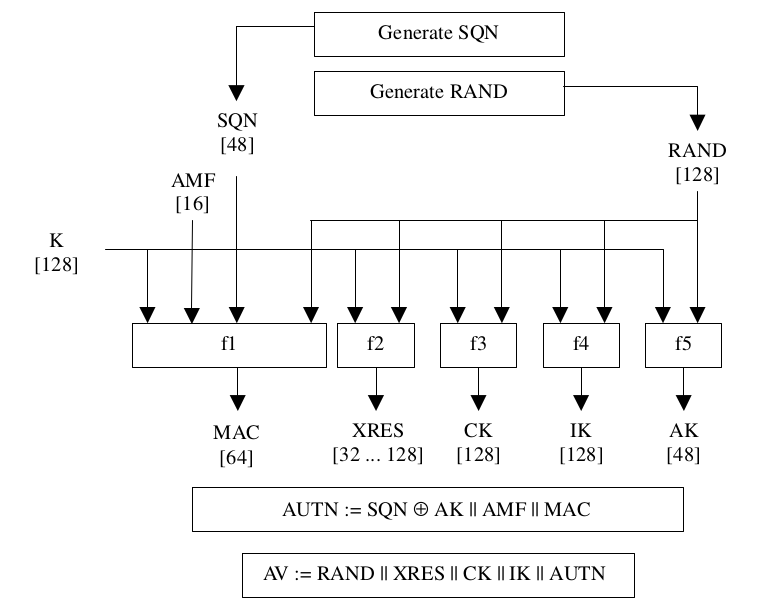
\includegraphics[width=300pt]{generation_of_authentication_vectors}
  \end{center}
  \caption{Übersicht über die Generierung der Authentifizierungsvektoren \cite{3gpp.33.102}}
  \label{fig:funktionsubersicht}
 \end{figure}
 
 In \Abbildung{funktionsubersicht} ist zu sehen, dass zu Beginn die \ac{SQN} generiert wird. Diese ist insgesamt 48 Bits lang und besteht aus den beiden Teilen SEQ und IND, mit SEQ als der die eigentliche Sequenznummer und IND als Arrayindex. Dieser Index wird benötigt, da auf der SIM-Karte sind die letzten SQNs in einem Array gespeichert. Die empfohlene Arraygröße ist 32, was für IND eine Länge von fünf Bits bedeutet. Mit diesem Index kann nachher die Aktualität der SEQ überprüft werden.\cite{3gpp.33.102} \\
 Für die Bildung der SEQ selbst gibt es drei verschiedene Möglichkeiten:
 \begin{itemize}
  \item teilweise zeitbasiert
  \item nicht zeitbasiert
  \item komplett zeitbasiert
 \end{itemize}
 
 Die einfachste Variante ist die nicht zeitbasierte Lösung, bei der lediglich ein Zähler hochgezählt wird mit jeder Authentifizierungsanfrage. Die SEQ ist initial also 0 und wird hochgezählt und gleichzeitig vom \ac{AuC} in einer Datenbank gespeichert \cite{3gpp.33.102}. Auf die anderen Möglichkeiten wird hier nicht näher eingegangen, da sie in dieser Arbeit keine Anwendung fanden.
 
 Als nächstes wird die \ac{RAND} gebildet. Das Verfahren, wie der Netzprovider diese RAND generiert darf nicht offen gelegt werden, da dies die Sicherheit stark beeinflussen würde. Generell handelt es sich dabei um eine 128-bit lange Zufallszahl, die für jede Funktion benötigt wird.
 
 \Abbildung{funktionsubersicht} zeigt zwar, welche Variablen in die Funktionen einfließen und welche Werte sie zurückgeben, aber sie zeigt nicht näher wie diese Werte nun verarbeitet werden. Dies zeigt \Abbildung{schematisch_milenage} besser. Dort ist zu erkennen, dass \emph{f2} bis \emph{f5*} nach dem selben Schema berechnet werden können und \emph{f1}, sowie \emph{f1*} noch einige zusätzliche Parameter haben.
 
 Zunächst die Erklärung der Symbole sowie einiger weiterer Abkürzungen. \ac{OPc} wird durch folgende Formel generiert:
 \begin{center}
  $OP_{C} = OP \oplus E(OP)_{K}$
 \end{center}
 
 $E()$ ist die Blockschiffrierung. In diesem Falle wird also \ac{OP} mit dem Schlüssel \ac{K} verschlüsselt. Welche Verschlüsselung gewählt wird, wird von 3GPP nicht vorgegeben. In dieser Arbeit wurde \ac{AES} verwendet, welche im Kapitel \Verweis{aes} näher beschrieben wird. \\
 Der verschlüsselte OP wird dann im zweiten Schritt über XOR ($\oplus$) mit dem ursprünglichen OP verknüpft.
 
 \begin{figure}[ht]
  \begin{center}
   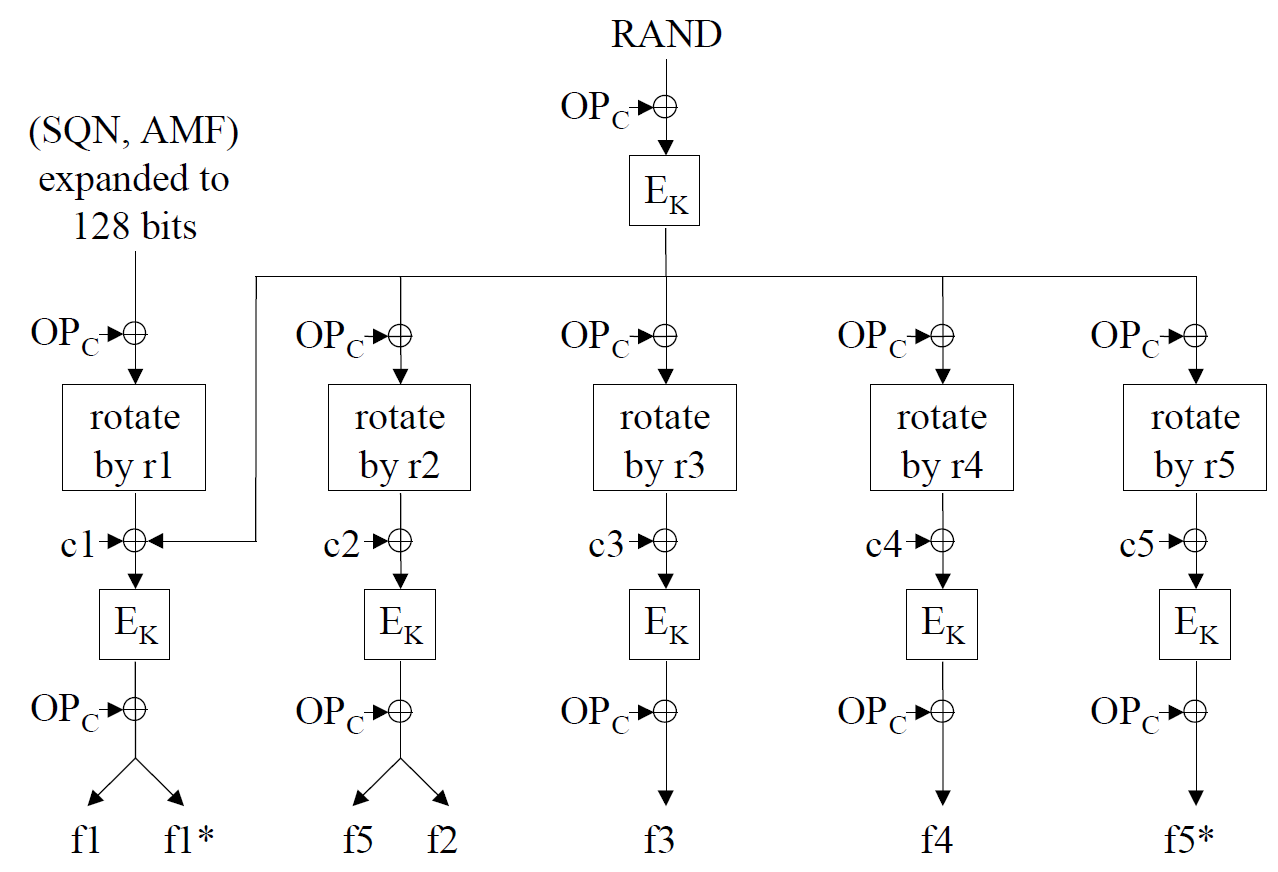
\includegraphics[width=400pt]{detailed_generation_of_authentication_vectors}
  \end{center}
  \caption{Schematische Darstellung zur Berechnung der Authentifizierungsvektoren \cite{3gpp.33.102}}
  \label{fig:schematisch_milenage}
 \end{figure}
 
 In \Abbildung{schematisch_milenage} ist weiterhin der Funktionsblock ``rotate by r'' zu lesen. Beim rotieren wird der Eingabewert um die Anzahl an Bits des Wertes von r rechts rotiert und die Bits die herausfallen links wieder eingefügt. Beispielsweise wird aus 110101 bei einem Rotationswert r von 2: 011101.
 
 Mit den genannten Infos ist verständlich, dass die Funktionen \emph{f2} bis \emph{f5*} ausgehen von einem verschlüsselten $RAND \oplus OP_{C}$, welcher in der Dokumentation auch als TEMP bezeichnet wird. Dieser Wert wieder wieder über XOR-mit $OP_ {C}$ verknüpft und um die entsprechende Rotationskonstante r rotiert. Im Anschluss wieder eine XOR-Verknüpfung mit der speziellen XOR-Konstante c und die Schiffrierung des Ausgabewertes. Im letzten Schritt wird dieser dann nochmal über XOR mit $OP_{C}$ verknüpft. \\
 Wie die \Abbildung{schematisch_milenage} zeigt funktionieren \emph{f1} und {f1*} sehr ähnlich. Bevor jedoch TEMP in die Berechnung einfließt wird SQN und AMF auf 128 Bits erweitert und bekommt in der Dokumentation die Bezeichnung IN1. IN1 besteht aus SQN und AMF abwechselnd konkateniert, also SQN $\|$ AMF $\|$ SQN $\|$ AMF. \cite{3gpp.33.102}
 
 
 \subsubsection{AES}
 \label{aes}
 
 \cite{paar09}
 
 \clearpage

\subsection{PPP}
Zur Bereitstellung einer Punkt-zu-Punkt-Verbindung als Grundlage des Authentifizierungsvorgangs
wird von Providern (\ac{ISP}) Implementierungen eines
\ac{PPP} verwendet. Mit Protokollen dieser Art wurden zum Beispiel schon Modem- oder ISDN-Verbindungen
aufgebaut. Heutige Szenarien sind unter anderem auch GPRS- und UMTS-Datenverbindungen -
hier hauptsächlich in
Form von \ac{PPPoE}. Auf beide Architekturen wird im folgenden
genauer eingegangen.



\subsubsection{Architektur PPP}
\ac{PPP} ist Teil der TCP/IP-Protokollsuite und sichert die komplette Funktionalität des
Datalink-Layers und wurde speziell für den Betrieb von Modems etc. entwickelt.
Jede Maschine, die ein Modem in Betrieb hatte, nutzte bereits \ac{PPP} um z.B.
Internet im lokalen Netzwerk freizuschalten und zu verteilen.
Neben der Freischaltung von Internetverbindungen wird \ac{PPP} von vielen \ac{ISP}
auch dazu verwendet Zugriffe zu monitoren sowie Angriffe durch Intrusion Detection zu vermeiden.
In üblichen \ac{LAN}-Umgebungen ist es notwendig, dass eingesetzte Technologien die Datalink-Layer-Funktion
implementieren und darüberhinhaus über einen MAC-Meschanismus verfügen, da verschiedene
Quellen/Ziele das selbe Medium teilen könnten. Dieser Regulierungsmechanismus ist bei \ac{PPP}
nicht notwendig, da es sich um eine Punkt-zu-Punkt bzw. Ende-zu-Ende-Verbindung handelt.
In jedem Fall handelt es sich um genau zwei Teilnehmer:
\begin{itemize}
	\item Quelle
	\item Ziel
\end{itemize}

Neben dem Datalink-Layer baut \ac{PPP} notwendigerweise auch auf der bestehenden Verbindung
auf dem Physical-Layer auf.

\paragraph{Motivation} Die Architektur ist gezielt sehr simpel gewählt. Es werden lediglich IP-Datagramme zwischen den
Endgeräten enkapsuliert. Vergleichbar ist der Aufbau mit dem von Ethernet, jedoch ohne
die notwendige Behandlung vieler Probleme die in sonstigen \ac{LAN}- und Breitbandumgebungen
auftreten können. So ist der Header z.B. nur 8 Byte statt 16 Byte lang. Doch dazu später mehr.
\ac{PPP} wurde als Alternative zum bereits bestehenden \ac{SLIP} implementiert, welches neben den notwendigen
Methoden, dem multiplexen verschiedener Netzwerklayer-Protokolle sowie mehrere Authentifizierungsmethoden noch zusätzliche Funktionen ermöglichte, die nicht benötigt werden.

\paragraph{PPP Frame}
Ein \ac{PPP}-Frame ist wie folgt aufgebaut:

\begin{itemize}
\item flag (1 Byte) - hexadezimal - Funktion des Paketdelimiter
\item address (1 Byte) - hexadezimal (FF) - Indikator für 'adressiert an alle Stationen'
\item control (1 Byte) - hexadezimal (03) -identifiziert Paket als \ac{HDLC}
\item protocol (2 Byte) - hexadezimal - identifiziert erwünschtes bzw. eingesetztes Protokoll
	\begin{itemize}
		\item 0xxx bis 3xxx : Netzwerklayer-Protokolle
		\item 4xxx bis 7xxx : Low Level Netzwerklayer Protokolle ohne \ac{NCP}
		\item 7xxx bis bxxx : Low Level Netzwerklayer Protokolle mit \ac{NCP}
		\item cxxx bis fxxx : Link Layer Protokoll wie LCP und zusätzliche Authentifizierungsprotokolle
	\end{itemize}
\item data and pad (variabel, maximal 1.500 Byte)
\item frame check sequence (2 Byte oder 4 Byte)
\item flag (1 Byte)
\end{itemize}

 \begin{figure}[htp]
  \begin{center}
   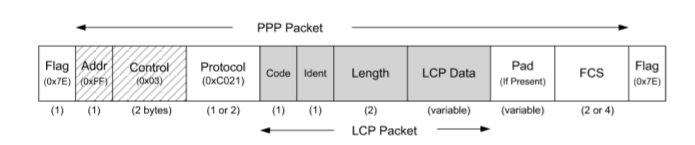
\includegraphics[width=500pt]{aufbau_ppp_frame}
  \end{center}
  \caption{Aufbau eines PPP-Frames}\cite{tcpipillustrated}
  \label{abb:aufbau_ppp_frame}
 \end{figure}

Diverse oben genannte Felder können in ihrer Länge variieren, da 
diese während des Verbindungsaufbaus vom \ac{LCP} ausgehandelt werden.

\paragraph{LCP Frame} Um die effizienteste Verbindungsart zu finden, benutzen PPP-Systeme
immer \ac{LCP} um die korrekten Parameter auszuhandeln. LCP-Nachrichten in ausgetauschten
PPP-Frames enthalten somit alle Konfigurationsoptionen für die sich gerade aufbauende
Verbindung. Ist eine Konfiguration gefunden, die beide Knoten unterstützen folgt der
Link-Establishment-Prozess. Ist dieser erreicht müssen danach keine weiteren redundanten
Paketinformationen im Header mitgetragen werden.

Ein LCP-Frame ist wie folgt aufgebaut:
\begin{itemize}
	\item code (1 Byte) - hexadezimal - enhält den Messagetyp (als Codes spezifiziert)
	\item identifier (1 Byte) - hexadezimal - mit diesen werden Anfragen bzw. Antworten mit einzelnen LCP-Transaktionen in Verbindung gebracht
	\item length (2 Byte) - hexadezimal - beinhaltet die Länge der Nachricht (inklusive code, identifier, length, data)
	\item data (variabel) - hexadezimal - Nutzdaten
\end{itemize}

\ac{LCP} ist so entworfen, dass Hersteller ihre eigenen Optionen einsetzen können, ohne
selbige explizit über \ac{IANA} spezifizieren zu müssen. Dokumentiert ist dies in \textbf{RFC2153}.

\paragraph{Aufbauphasen} Nachfolgend werden die verschiedenen Aufbauphasen des
PPP-Protokolls erläutert. Im \Anhang{abb:aufbauphasen_pppverbindung} befindet
sich eine Abbildung, die diesen Vorgang illustriert.

\textbf{Link Dead Phase:}
Beide Systeme fangen mit dieser Phase an und enden hiermit wieder.
Grundlage ist, dass außer (maximal) dem Link auf physischer Ebene,
keine Verbindung zwischen beiden Endpunkten besteht. Normalerweise
wird nach sicherstellen des physischen Links von einer Seite der
Aufbau der Verbindung initiiert. Dies geschieht meist mit einer Form von Modem.
Nach Abschluss der Initiierung beginnt die nachfolgende Phase.

\textbf{Link Establishment Phase:}
Das initiierende System System sendet eine \ac{LCP}-Nachricht an das Zielsystem,
um Optionen anzufordern, die gesetzt werden sollen. Dazu gehören
Netzwerklayer-Protokoll, Authentifizierungsmethode und andere optionale
Funktionen. Sofern das Zielsystem alle angeforderten Optionen beherrscht,
kann dieses eine Bestätigung (\textbf{ACK}) an das Quellsystem senden.
Ist dies nicht der Fall, wird eine Anwort verfasst, die sowohl alle
\textit{nicht unterstützten} als auch alle \text{unterstützten} Optionen
enthält, damit das Quellsystem nach Empfang dieser Information eine
Verbindung initiieren kann, die in jedem Fall von beiden Seiten unterstützt
wird. Das erfolgreiche Abschließen dieser Phase führt zur nächsten Phase.

\textbf{Authentication Phase:}
Diese Phase ist optional. Ausgelöst wird sie durch das vorhandensein einer
Authentifizierungsoption in der LCP-Konfigurationsnachricht.
Zur Auswahl stehen z.B. \ac{PAP} oder \ac{CHAP}.
Hierbei greift PAP auf Username und Passwort, CHAP auf eines komplexeren Informationsaustausch
mit einem Challenge-Response-Verfahren zurück. Wobei der Erfolg immer zu nächsten
Phase führt ist die Reaktion bei Misserfolg des Vorgangs Protokollabhängig.

\textbf{Link Quality Monitoring:}
Diese Phase ist wie ihr Vorgänger ebenfalls optional - ebenfalls ausgelöst durch
die gewählt Option in der LCP-Nachricht.
Hier aus mehreren Protokollen gewählt werden. Eines davon ist standardisiert:
das 'Link Quality Report Protocol'. Registriert werden unter anderem der Linktraffic
sowie Fehlermeldungen.

\textbf{Network Layer Protocol Configuration:}
Wie bereits erwähnt unterstützt PPP  das multiplexen von Protokollen auf
Netzwerklayerebene. Für jedes einzelne, das eingesetzt wird,
führt das System einen separaten Prozess des Verbindungsaufbaus durch.
Jedes Netzwerklayerprotokoll verfügt über einen eigenes \ac{NCP} sowie \ac{IPCP}.
Vergleichbar ist dies mit dem Aufbau von \ac{LCP} - nur spezifischer.

\textbf{Link Open Phase:}
Nachdem alle individuellen Optionen und NCP-Exchanges erfolgreich durchgeführt wurden,
ist der Verbindungsaufbau komplett und Protokolldaten können jetzt über den aufgebauten
Link in beide Richtungen ausgetauscht werden.

\textbf{Link Termination Phase:}
Wird die Verbindung absichtlich (Ablauf der Session, Authentifizierungsfehler)
oder durch Fehler o.ä. physikalisch getrennt, wird im Regelfall über \ac{LCP}
eine 'Terminate Request Message' versandt. Diese kann von der Gegenseite
angenommen (\textit{AKC}) werden, sofern die grundlegende Verbindung noch aktiv ist.
Beide Systeme sind dann wieder in der ursprünglich genannten 'Link Dead Phase'.
Eine Terminierung der Verbindung ist neben \ac{LCP} auch auf \ac{NCP}-Ebene möglich,
damit die PPP-Verbindung trotz 'Terminierung' bestehen bleibt.


\subsubsection{Architektur PPPoE}
Zur Realisierung der Verbindung zwischen Authentifizierungsstelle und
Endgerät wurde aufgrund der Beschaffenheit des Raspberry Pis eine
Ethernetverbindung gewählt. Dieser wird das im vorangegangenen
Abschnitt erläuterte \ac{PPP}-Protokoll zugrunde gelegt.
In Ethernetframes werden PPP-Daten als Nutzdaten enkapsuliert.
Diese Methode wurde auch im realen Umfeld dazu entwickelt \ac{ISP}s die
Möglichkeit zu geben Verbindungen über Kabelmodem oder DSL in Form
von Bridged-Topologien zu realisieren. Provider bewerkstelligen
so auch die Endpunktidentifikation, Accounting und Rechnungserstellung.
(Beschrieben wird der Standard in RFC2516)

\paragraph{Aufbauphasen}
im Kontext einer PPPoE-Verbindung sind Discovery und Session.
Beide werden nachfolgend erläutert.

\paragraph{Discovery}
ist die Phase, in der der Client PPPoE-Frames dazu verwendet einen
Zugangspunkt zu finden.

Dies geschieht in den folgenden Schritten bzw. Frames:
\begin{enumerate}
\item PPPoE Active Discovery Initiation (PADI) - Ein Frame, vom Client
      gesendet an die Broadcastadresse 0xFF-FF-FF-FF-FF-FF.
      Falls vorhanden, werden weitere Parameter als Payload 
      mitgeschickt. (Codefeld:9; Session-ID:0)
\item PPPoE Active Discovery Offer (PADO) - Ein Frame, der von der
      Authentifizierungsstelle an die Unicast MAC-Adresse des
      initiierenden Client geschickt wird. Weitere Parameter wie
      Service-Name o.ä. können ebenfalls mitgeschickt
      werden. (Codefeld:7; Session-ID:0)
\item PPPoE Active Discovery Request (PADR) - Ein Frame, der vom Client
      an die Unicat MAC-Adresse der Authentifizierungsstelle geschickt
      wird. (Codefeld:25; Session-ID:0)
\item PPPoE Active Discovery Session-Confirmation (PADS) - Ein Frame,
      der von der Authentifizierungsstelle an die Unicast MAC-Adresse
      des Client geschickt wird. Er enthält alle ausgehandelten Daten
      mit der zugewiesenen Session-ID. (Codefeld:101; Session-ID:XX)
\item PPPoE Active Discovery Terminate (PADT) - Ein Frame,
      der von beiden Endpunkten geschickt werden kann. Er signalisiert
      die gewünschte Verbindungsterminierung des Absenders.
      (Codefeld:167)
\end{enumerate}

\paragraph{Session}
ist die Phase, in der die PPPoE-Verbindung bereits erfolgreich
aufgebaut ist und Daten ausgetauscht werden können.
Dieser Zustand ist erreicht, sobald die PPPoE-Discovery-Phase
erfolgreich abgeschlossen ist.

<PPP-Daten im Ethernet Frame Abb?>

\subsection{Raspberry Pi}

Die Hardwaregrundlage für das Endgerät bietet die Plattform eines Raspberry Pis, einem Kleincomputer.

\subsubsection{Raspberry Pi Foundation}
Entwickelt wird der Raspberry Pi von der Raspberry Pi Foundation\footnote{\url{https://www.raspberrypi.org}}
(registriert in Großbritannien). Ziel der Organisation ist es,
seit Veröffentlichung des ersten Modells, einen kostengünstigen
Computer vorrangig für Bildungszwecke zu entwerfen. Auf diesem
Weg soll sowohl Erwachsenen als auch Kindern der Zugang zum
Programmieren oder anderen wissenschaftlichen Anwendungsgebieten
erleichtert werden.

Bisher wurden seit der initialen Veröffentlichung im Februar 2012(\cite{rasppifoundweb})
drei Generationen in unterschiedlichen Ausführungen
entwickelt. Die Bezeichnung A(+) bzw. B(+) gibt jeweils Aufschluss
über die jeweilige Ausführung.

\subsubsection{Hardware Modell B}
Das eingesetzte Modell B der ersten Generation verfügt über folgende Hardwarekomponenten:
\begin{itemize}
\item CPU - 700 MHz Singlecore ARM1176JZF-S
\item RAM - 512 MB
\item Speicherslot - SDHC
\item Grafikprozessor - Broadcom VideoCore IV
\end{itemize}

\subsubsection{Betriebssystem}
Als Betriebssystem gibt es für den Raspberry Pi eine breite Auswahl.
Neben einer Vielzahl von Media-Center-Plattformen sind auch alle
Desktop- bzw. Server-Versionen gängiger Linux-Derivate verfügbar:
Arch Linux, Puppy Linux, Raspbian, openSUSE, Gentoo Linux, Ubuntu Mate,
CentOS, Slackware, ...

\paragraph{Raspbian}
Aufgrund hoher Stabilität und Verfügbarkeit aller benötigten Treiber
(u.a. dem SIM-Kartenleser) wurde die auf \textit{Debian GNU Linux}\footnote{\url{https://www.debian.org/}}
basierende Distribution \textit{Raspbian}\footnote{\url{https://www.raspbian.org/}} ausgewählt.
Es erbt somit alle Eigenschaftem vom übergeordneten Debianprojekt.
So auch den Paketmanager \textit{dpkg} mit ca. 35.000 vorkompilierten
Softwarepaketen - in einigen Fällen für den Betrieb mit dem
Raspberry Pi optimiert. Nicht vorpaketierte Software kann auf dem Raspberry
Pi durch vorhandensein einer Vielzahl von Libraries und Build-Tools
für die ARM-Architektur kompiliert werden.

Über den rein funktionalen Konsolenbetrieb hinaus, wird Raspbian standardmäßig mit den
Windowmanagern XFCE oder LXDE ausgeliefert.

Nachdem im Juni 2012(\cite{raspbianweb}) die erste
Version fertiggestellt wurde ist Raspbian nach wie vor aktiv
in Entwicklung. Momentan im stabilen Debian-Release \textit{Jessie}.
Selbiges wird auch zur Umsetzung des Endgerätes eingesetzt.
Die vorkompilierten Pakete stammen dementsprechend aus dem aktuellen
\textit{stable}-Zweig, der häufig vor allem im Umfeld des Serverbetriebes
anzutreffen ist. Die Ursache hierfür ist die Tatsache, dass das
Projekt Pakete erst nach einem langen Testprozess im \textit{unstable}-
sowie darauffolgenden \textit{testing-}Zweig für den \textit{stable}-Zweig
freigibt. Im Kontrast zu gängigen Desktop-Distributionen, die
im Vergleich zu Debian stärker auf Aktualität achten.

Neben den Zielen der Raspberry Pi Foundation verfolgt das Projekt
auch die Ziele des Debian/GNU-Projekts. Es ist dementsprechend unter
den \textit{Debian Free Software Guidelines}\footnote{\url{https://wiki.debian.org/DFSGLicenses}} lizensiert und durch die Raspbian-Community unabhängig
entwickelt.

\subsection{pysim}

\subsection{Die Sprache C}

\subsection{Projektspecs}

\section{Tätigkeit}
	\subsection{Erstellen des Netzproviders}
		\subsubsection{Ubuntu}
		Wie in \Verweis{subsec:ubuntu} beschrieben wird Version 14.04 LTS
		der Linuxdistribution Ubuntu installiert. Das bei der Herstellerwebsite\footnote{\url{http://releases.ubuntu.com/14.04/}},
		für Serverbetrieb erhältliche Image wird in einer virtuellen Maschine installiert.
		Diese weist folgende Eigenschaften auf:

		\begin{tabularx}{\textwidth}{|l|X|}
    	\hline
      		\textbf{Gerät} & \textbf{Typ} \\
    	\hline
    	\hline
    		CPU & 1x 64 Bit \\
    	\hline
    	\hline
    		RAM & 1x 1024 MB \\
    	\hline
    	\hline
    		HDD & 1x 10 GB \\
    	\hline
    	\hline
    		NIC & 2x Bridged (1x auf enp0s25; 1x auf wlp3s0) \\
    	\hline
    	\end{tabularx}

    	Aufgrund der Tatsache dass nur ein einziger Client übder den Zugang von \textit{PPPoE}
    	zu erwarten ist, sind die Anforderungen an CPU, Arbeits- und Festplattenspeicher
    	recht gering. Wichtig ist das Vorhandensein zweier Netzwerkschnittstellen, die
    	auf jeweils eine physikalisch Schnittstelle geleitet werden. Dies ist notwendig,
    	da sowohl die \ac{MS} über eine Ethernetverbindung mit der virtuellen Maschine angebunden sein,
    	als auch eine Dauerhafte Internetverbindung mit der verbleibenden Schnittstelle
    	aufrecht erhalten werden muss. So ist es möglich nach erfolgreicher Authentisierung
    	des \ac{MS} den Zugang zum Internet freizuschalten.

    	\subsubsection{PPPoE}
    	kann nach der vollständigen Ubuntuinstallation durchgeführt werden. Hierzu wird die aktuelle
    	Version 3.11 auf der Herstellerwebsite\footnote{\url{https://www.roaringpenguin.com/products/pppoe}}
    	heruntergeladen und auf dem Server entpackt. Zusätzlich wird das Ubuntu-Paket zur Unterstützung
    	des Point-To-Point-Protocol (als \textit{ppp} erhältlich) benötigt. Sind diese beiden Grundvoraussetzungen
    	abgedeckt wird der Roaring Penguin PPPoE-Server ohne spezielle Änderungen kompiliert.

    	In der Datei \textit{/etc/ppp/pppoe-server-options} werden die Parameter gesetzt. Anzugeben
    	sind die DNS-Server sowie die CHAP-Authentifizierung. Der User für die Authentifizierung
    	wird unter \textit{/etc/ppp/chap-secrets} definiert.

    	Der zu verwendende Adresspool an IP-Adressen ist unter \textit{/etc/ppp/allip} anzugeben.

    	Abschließend fehlt noch die Deklaration der zu verwendenden Netzwerkschnittstelle (unter \textit{/etc/network/interfaces}),
    	die zum Betrieb mit PPPoE eingesetzt werden soll. Ihr muss eine valide IP-Adresse aus dem definierten
    	Pool sowie eine Subnetzmaske zugewiesen werden.

    	Alle Konfigurationsdateien befinden sich im Anhang. %TODO: #edit Anhang pflegen

    	Damit die Internetverbindung nach erfolgreicher Authentifizierung des \ac{MS} auch
    	korrekt von Provider freigeschaltet und weitergeleitet wird, muss eine IPTables-Regel
    	eingerichtet werden:

    	\begin{lstlisting}[language=bash]
  			$ iptables -t nat -A POSTROUTING -s 192.168.178.0/24 -o enp0s25 -j MASQUERADE
		\end{lstlisting}

		Sie nimmt den Verkehr auf dem Device \textit{enp0s25} an und maskiert (\ac{NAT}) diesen
		für den weiteren Betrieb (wie es bei einem realen Provider auch wäre). Dies geschieht
		für eingehenden sowie ausgehenden Verkehr. Die auf den zweiten Netzwerkadapter geleitete
		Netzwerkschnittstelle bleibt mit Defaultwerten konfiguriert und fungiert als Zugangspunkt
		zum Internet.

		\subsubsection{Implementierung Milenage}
		\subsubsection{Implementierung AES}
			\paragraph{'Unter'-Algorithmen}
	\subsection{Erstellen des UE}
		\subsubsection{Aufsetzen des Pis}
			\paragraph{rasbian}
			\paragraph{pysim}
	\subsection{Integration mit PPPoE}
		 \subsubsection{roaring penguin pppoe}

\clearpage
\section{Ergebnis}
	Die beiden nachfolgenden Kapitel beschäftigen sich mit der Offenlegung durchgeführter Tests und deren Ergebnisse.
	Hierbei wird näher darauf eingegangen für welche Teilaspekte welche Prüfmechanismen
	eingesetzt wurden. Ebenso wird verdeutlicht, welche Funktionen erfolgreich, beziehungsweise
	mit zwischenzeitlichen Komplikationen implementiert werden konnten.

	\subsection{Funktionsprüfung}
	\label{ergebnis-tests}
	Nachfolgende Tabelle liefert zunächst eine Übersicht zu implementierten und im Anschluss
	getesteten Funktionen:\vspace*{5mm}

	\begin{table}[h]
	\begin{tabularx}{\textwidth}{|X||X|X|}
    \hline
      \textbf{Funktion} & \textbf{Komplikationen bei Integration bzw. Implementierung} & \textbf{Abschließender Erfolg} \\
    \hline
    \hline
     	Bereitstellung des Raspberry Pis (UE) & $\bullet$ & $\checkmark$ \\
    \hline
    \hline
     	Bereitstellung der virtuellen Maschine (Provider) & $\circ$ & $\checkmark$ \\
    \hline
    \hline
     	Entwicklung AES & $\bullet$ & $\checkmark$ \\
    \hline
    \hline
    	Entwicklung Milenage & $\bullet$ & $\checkmark$ \\
    \hline
    \hline
    	Integration SIM-Karte und SIM-Kartenleser & $\circ$ & $\checkmark$ \\
    \hline
    \hline
    	Entwicklung Client/Server-Kommunikation & $\bullet$ & $\checkmark$ \\
    \hline
    \hline
    	Integration PPPoE (Client und Server) & $\circ$ & $\checkmark$ \\
    \hline
    \hline
    	Integration aller Komponenten zur Authentisierung & $\bullet$ & $\checkmark$ \\
    \hline
    \end{tabularx}
    \caption{Ergebnisse der Funktionsprüfung}
    \end{table}

    \centerline{$\bullet$=eingetreten; $\circ$=nicht eingetreten; $\checkmark$=Erfolg; \ding{55}=Misserfolg}\vspace*{5mm}

    Wie Tabelle 5 zu entnehmen ist, konnten alle gewünschten Funktionen sichergestellt werden.
    Welche Komplikationen auftraten und mit welchen Mitteln diese behoben wurden, ist im
    nächsten Kapitel beschrieben (vgl. \Verweis{subsec:fehler}).


		\subsubsection{AES}
		Wie bereits unter Kapitel \Verweis{implementierung-aes} erläutert, basierte die Implementierungsphase
		primär auf der Entwicklung der \textit{AES}-Verschlüsselung. 

		Während der Implementierung wurde das Tool AES-Vizualization\footnote{\url{http://www.cs.mtu.edu/~shene/NSF-4/AES-Downloads/index.html}} eingesetzt (vgl. \Verweis{subsubsec:aesviz}).
		Dieses ermöglicht es den \textit{AES}-Algorithmus schrittweise zu durchlaufen.
		Um die Korrektheit der Implementierung nachzuvollziehen wurde der \textit{Practice-Mode}
		des Tools verwendet. Nach dem Start des Tools werden zwei Testwerte für den
		Eingabetext sowie den CypherKey generiert. Diese wurden jeweils in die eigene
		Implementierung übertragen und dann alle Folgeschritte geprüft.

		Auf diesem Weg konnten alle Funktionen vom \textit{SubBytes}, über \textit{ShiftRows},
		\textit{MixColumns}, \textit{AddRoundKey} bis hin zum \textit{KeySchedule} erfolgreich verifiziert
		werden.

		Zusätzlich wurden einige Testvektoren, die von Vladimir Klykov veröffentlicht
		wurden\footnote{\url{http://www.inconteam.com/software-development/41-encryption/55-aes-test-vectors\#aes-ecb-128}}
		testweise übernommen und geprüft. Hier wird immer statisch ein Eingabetext sowie ein
		Cypherkey gelistet, mit dem die Verschlüsselung getestet werden kann. Der Vergleich
		der generierten Cyphertexte gibt dann Aufschluss darüber ob die Implementierung
		wie erwünscht arbeitet.


		\subsubsection{Milenage}
		Der Austausch verschiedener, generierter bzw. auch statischer Werte zwischen eigenem
		Implementierung und der SIM-Karte konnte mit \textit{UMTS Security Algorithms}
		von Fabricio Ferraz\footnote{\url{http://fabricioapps.blogspot.de/2011/05/umts-security-algorithm-milenage.html}}
		geprüft werden. Das Tool wurde auf Empfehlung von Herrn. Prof. Dr. Müller eingesetzt.

		Besonders hilfreich ist die Ausgabe aller Zwischenergebnisse von Teilfunktionen
		\textit{f1}-\textit{f5} sowie \textit{AUTN}, \textit{Kc} und \textit{SRES} auf
		den Seiten beider Teilnehmer. Auf diesem Weg konnten alle festen (geheimen) sowie
		dynamisch generierten Werte in das Tool eingesetzt und Ergebnisse Schritt für
		Schritt verifiziert werden. Bei auftretenden Fehlern im Endergebnis konnten Ursachen
		genauer eingegrenzt und behoben werden.

		\subsubsection{SIM-Karte und SIM-Kartenleser}
		Diese beiden Komponenten konnten direkt nach der Treiberintegration im Betriebssystem
		geprüft werden.

		Die Funktionalität des Treibers konnte durch ein entsprechendes identifizieren des
		Betriebssystems in Form eines PC/SC-Gerät sichergestellt werden.

		Teiberinterne Scan-Mechanismen gaben Auskunft über das Vorhandensein einer SIM-Karte,
		sowie rudimentäre Abfragen. So kann z.B. die IMSI direkt ausgelesen werden.

		\subsubsection{Client- und Server-Kommunikation}
		Die Kommunikation zwischen Client- und Server-Komponenten wurden über die bereits zuvor
		fertiggestellte Implementierung der jeweiligen Gegenseite getestet.

		Auf der Seite des Providers (AuC) wurden zuerst die erwarteten Werte der SIM-Karte, sowie
		das Initiieren der Authentifizierung hart kodiert. Hierbei wurde natürlich die spätere
		Reihenfolge des Authentifizierungsvorgangs eingehalten. Nach Sicherstellung dieses Vorgangs
		konnten umgekehrt die Antworten beziehungsweise Anfragen des Providers auf der Seite des Teilnehmers
		simuliert werden. Ebenfalls hart kodiert.

		Im Anschluss daran wurden beide Teilkomponenten im realen Umfeld verbunden und der
		Authentifizierungsablauf erneut geprüft.

		\subsubsection{PPPoE}
		Der ordnungsgemäße Aufbau der PPPoE-Verbindung ließ sich durch die diensteigene
		Log-Ausgabe verfolgen. Nach dem Start des Serverdienstes gibt dieser Auskunft
		darüber, ob jetzt einkommende Verbindungen erwartet werden.

		Aus der Sicht des Clients konnten ebenfalls Logdateien verwendet werden.

		Nach erfolgreichem Verbindungsaufbau war es möglich die vorhandene
		IP-Tables-Route zu prüfen. Mit der Auslieferung von Ressourcen aus
		dem Internet war auch diese Funktion über PPPoE sicherzustellen.

	\subsection{Fehler}
	\label{subsec:fehler}
		\subsubsection{Einrichtung verwendeter Werkzeuge}
			\paragraph{Raspbian} konnte ohne Probleme installiert und in
			Betrieb genommen werden (vgl. \Verweis{subsubsec:installpi}). Der einzige Zwischenfall ist auf eine
			defekte SD-Speicherkarte zurückzuführen. Nach wenigen Wochen
			des Betriebes ist diese ausgefallen, was ein starten des
			Raspberry Pis unmöglich machte. Ebenfalls konnten die auf der
			Speicherkarte enthaltenen Daten nicht wieder hergestellt werden.

			Aus diesem Grund war es notwendig das Betriebssystem erneut aufzusetzen.
			Eingeleitete Gegenmaßnahme für zukünftige Ausfälle war ein regelmäßiges Backup
			nach Änderungen am System. Via \textit{dd} wurde immer blockweise ein komplettes Abbild
			des aktuellen Systems auf externen Festplattenspeicher übertragen.

			Es blieb bei einem einzigen Hardwareausfall der SD-Karte.

			\paragraph{Ubuntu} konnte ohne Probleme installiert sowie betrieben werden.
			Schon in der Standardinstallation des Server-Images können Netzwerkschnittstellen,
			von Virtualbox bereitgestellt und direkt konfiguriert beziehungsweise auch genutzt werden.

		\subsubsection{Fehleinschätzungen}
		Die meisten und gravierendsten Fehleinschätzungen beziehungsweise Probleme
		wurden während der Inbetriebnahme der Karte sowie der Entwicklung
		der Softwarekomponenten aufgedeckt.

		\paragraph{pysim}
		Die erste Fehleinschätzung war der Einsatz des Tools pysim, welches
		primär zu ersten Test in der Kommunikation mit der vorliegenden
		SIM-Karte angedacht war. Es stellte sich während der Implementierungsphase
		als problematisch heraus, da es nicht über alle der benötigten 
		Funktionalitäten verfügt. Zwar konnte mit pysim ein erster
		Kommunikationsversuch erfolgreich gestartet und abgeschlossen werden,
		nicht jedoch eine Authentifizierung initiiert werden. Dies lag
		vor allem, dass die beiden Verfassern dieser Studienarbeit sich nicht
		sicher waren welche Art der Authentifizierung angewandt werden muss.
		Die für eine GSM- oder UMTS-fähige SIM-Karte.

		Bei ersten Tests mittels pysim wurde schnell deutlich, dass es
		sich um eine UMTS-Authentifizierung handeln muss. Die vorliegende
		Python-Bibliothek pysim ist jedoch nicht dazu in der Lage diese
		Art von Authentifizierung zu initiieren. Wie unter \Verweis{subsec:pysim}
		genauer erläutert konzentriert sich pysim von Kevin Prince auch
		eher auf die Programmierung entsprechender SIM-Karten, statt
		dem universellen auslesen dieser.

		Nachdem sich herausstellte, dass \ac{UMTS}-Kartensupport ebenfalls 
		notwendig ist, fiel die Alternativwahl
		auf die Bibliothek \textit{osmo-sim-auth} eingesetzt
		(vgl. \Verweis{subsec:osmosim}). Über diese Bibliothek konnten
		alle Funktionen auf der Seite des UE in der Sprache Python
		implementiert werden.

		\paragraph{AUTN} Unsicherheiten enstanden auch bei ersten Testdurchläufen
		mit \textit{osmo-sim-auth}. Da zu diesem Zeitpunkt noch keine 
		vollständige Implementierung zur Generierung aller benötigten
		Werte existierte, wurde die Zusammensetzung für den
		Parameter \textit{AUTN} zufällig gesetzt. Dies resultierte jedoch
		darin, dass die SIM-Karte einen Fehler zurück lieferte. Mit
		Analyse des Fehlercodes \textit{SW 98 62} wurde schnell klar,
		dass die Zusammensetzung des Parameters \textit{AUTN} zwingend
		den Vorgaben entsprechen muss, um korrekt zu funktionieren.

		Nach der Fertigstellung der Implementierung konnte der Test erneut
		durchgeführt werden. Dieses mal mit Erfolg. Die SIM-Karte lieferte
		einen generierten Wert zurück: \textit{AUTS}.

		\paragraph{Resynchronisation der SQN} Während die verbleibende
		Implementierungsphase weitestgehend wie geplant verlief, zeichnete
		sich kurz vor Abschluss der Phase ein weiteres Defizit im Code ab.

		Mit der bereits erläuterten Milenage-Prüfsoftware konnten fast
		alle berechneten, übertragenen sowie von der SIM-Karte empfangenen
		Werte korrekt verifiziert werden. Ausgehend von den festgelegten
		Geheimnissen \textit{K}, \textit{OP(c)}, dem ausgetauschten \textit{RAND}
		über die berechneten Variablen \textit{f1-f5} bis hin zu \textit{Kc} sowie
		\textit{SRES} auf beiden teilnehmenden Seiten.
		Der Vergleich dieser Werte deutete darauf hin, dass die Implementierung
		korrekt sein muss.

		Problematisch war jedoch die Integration des Codes in die bereitstehende
		Umgebung. Während die Übertragung der Werte plangemäß verlief, antwortete
		die SIM-Karte nicht mit den erwarteten Vektoren \textit{CK}, \textit{IK}
		und \textit{Kc}, sondern lediglich mit einem einzigen Wert. Dieser
		stellte sich nach wiederholter Recherche in den 3GPP-Dokumenten als
		\textit{AUTS} heraus, welcher zur Resynchronisation der \textit{SQN}
		benötigt wird (vgl. \Verweis{par:resynchronisation}).

		Selbige Resynchronisation wurde im entwickelten
		Protokoll beziehungsweise Authentifizierungsvorgang bis zu diesem Zeitpunkt
		nicht berücksichtigt. Nach der Identifikation dieses Defizits
		konnte bei der Implementierung nachgebessert werden.

		Alle erforderlichen Informationen waren der Standardisierung
		durch die \textit{3GPP} zu entnehmen. Mit dieser Grundlage konnten
		notwendige Parameter aus der übermittelten \textit{AUTS} extrahiert
		und weiterverarbeitet werden, sodass die \textit{SQN} erfolgreich
		resynchronisiert wird. 

		Mit der Integration dieser Funktion könnten auch erfolgreich die
		Vektoren \textit{CK}, \textit{IK} und \textit{Kc} generiert werden.

\clearpage
\clearpage

\section{Diskussion}
\label{diskussion}

	\subsection{Alternative Vorgehensweisen}
	\label{diskussion-alternative}
	
	Die Arbeit ließ einiges an Spielraum besonders die Art der Umsetzung. Deshalb soll in
	diesem Kapitel aufgezeigt werden, was alternativ möglich gewesen wäre.
	
	Eine Möglichkeit wäre sicherlich gewesen für beide Seiten, also UE und AuC, die selbe
	Programmiersprache zu verwenden. So hätte beides mit C geschrieben werden können,
	jedoch wäre der Aufwand ein größerer geworden. Das liegt daran, dass für C keine
	Wrapper-Klasse in dem Umfang von pyscard (vgl. Kapitel \Verweis{pyscard}) existiert.
	Somit müssten einige Dinge, die durch pyscard und osmo-sim-auth abgewickelt wurden,
	selbst programmiert werden. Aber die Funktionalität wäre grundsätzlich durch PCSClite
	gegeben die USIM über C anzusprechen. \\
	Umgekehrt wäre die Möglichkeit gewesen den Netzprovider ebenfalls in Python zu
	implementieren. Die Fähigkeiten von Python wären für die Aufgabe ausreichend gewesen,
	zumal keine Optimierung auf Größe oder Geschwindigkeit des Programms gelegt wurde.
	Durch seine Hardwarenähe hat C in beiden Bereichen gegenüber Python einen Vorteil,
	aber diese war nicht gefragt. Jedoch hätte es bei Python das Problem gegeben, dass
	die vorhanden Kenntnisse sehr gering waren im Gegensatz zu C. Hier wäre also zu Beginn
	ein größerer Aufwand entstanden die Sprache zu lernen. \\
	Da das Programm zur Steuerung der SIM-Karte sehr geil ist, ist es jedoch kein Widerspruch
	hier die Zeit für die Grundkentnisse in Python zu investieren, da sie vermutlich geriger
	waren als der Zeitaufwand, der für eine Implementierung in C nötig gewesen wäre.
	
	Abschließend ist zu sagen, dass die Liste der Sprachen aus der gewählt werden konnte
	ziemlich umfangreich ist, aber mit pyscard existiert ein guter Wrapper für PCSClite und
	es ergab Sinn ein Projekt was mit Hardware kommuniziert auch mit einer hardwarenahen
	Sprache umzusetzen.	
	
	\subsection{Ausblick}
		\subsubsection{Verbesserungen}
		Wie in Kapitel \Verweis{ergebnis-tests} angesprochen wurde, sind alle gesetzten
		Ziele erreicht worden, aber es gab hier und da einige Probleme, die aufgetreten
		sind und manche von denen wären vermutlich vermeidbar gewesen. Dazu zählen vor
		allem Fehler bei der Entwicklung des AES- und Milenage-Algorithmuses.
		
		Lange bestand eine unterschiedliche Meinung darüber, wo der Unterschied von UMTS-
		und GSM-Authentifizierung lag. Und trotz vermehrter kurzer Unterhaltungen in
		denen dies offensichtlich wurde, hat es lange gedauert bis ein längeres Gespräch
		stattfand in dem gemeinsam geklärt wurde, wie sich beide unterscheiden. Wäre
		dieser Diskurs schon früher geführt worden, wäre eine erste Implementierung mit
		pysim vermutlich nicht geschehen, sondern die Suche wäre weiter gegangen und
		schon früher auf osmo-sim-auth gefallen.
		
		Der andere große Punkt war, dass nicht bekannt war, wie und wer den Wert von SQN
		verantwortet. Der Wert tauchte zwar immer wieder auf, aber in den Dokumenten,
		die gelesen wurden war dieser Wert im Gegensatz zu allen anderen nicht näher
		spezifiziert. Deshalb wurde zu Beginn angenommen, dass der Netzprovider SQN
		entscheidet und durch den AUTN die SIM-Karte diesen vermittelt bekommt. Es
		stellte sich jedoch raus, dass SQN von der USIM verwaltet wird und es sehrwohl
		eine Methode zur Berechnug der SQN gibt, aber es wurde an den falschen Stellen
		danach gesucht und versuchte deshalb kurz vor Projektabschluss nochmal Probleme.
		Ein Lesen der Referenzen der Milenage-Spezifikation 35.205 vom 3GPP hätte direkt
		zu dem Dokument 33.102 geführt, in der auch die SQN erläutert wurde. Hier gilt
		es beim	nächsten Mal nicht erst Google für die Suche zu bemühen sondern das zu
		durchsuchen, was schon existiert.
		
		\subsubsection{Mögliche zukünftige Projekte}
		Die Authentifizierung und der Schlüsselaustausch von UMTS ist noch umfangreicher
		als was in diesem Projekt umgesetzt wurde. Da es in diesem Projekt allein um die
		Authentifizierung ging, wurde die Berechnung von CK und IK vernachlässigt. Dies
		wäre in einem weiteren Schritt eine Möglichkeit. Dadurch könnten dann auch
		Nachrichten zwischen Nutzergerät und Authentifizierungsstelle verschickt werden.
		Noch ein Schritt weiter wäre eventuell eine weitere SIM-Karte, die sich beim
		Netzprovider authentifiziert und dann mit der jetzten USIM kommuniziert.

		Für diesen Schritt müsste jedoch vorher das Programm auf dem AuC angepasst
		werden und eine Datenbank erhalten, in der die unterschiedlichen Parameter für
		die einzelnen USIM's abgespeichert werden.

		Generell erlaubt der aktuelle Prozess nur USIM-Karten. Hier wäre zu überlegen
		für SIM-Karten auf dem GSM-Standard ebenfalls die
		Authentifizierung zu ermöglichen. Der Milenage-Algorithmus ermöglicht die
		Abwärtskompatibilität, weshalb kein neuer Standard verstanden werden muss und
		der zusäzliche Programmieraufwand nicht sehr groß sein wird.
	
		Generell sollte auch der Programmcoode optimiert werden. An einigen Stellen
		können Programmteile in eigne Funktionen ausgegliedert werden, um Redundanzen
		zu vermeiden und das Programm selbst im Speicherplatzverbrauch zu reduzieren. Des
		weiteren wird schon jetzt eine ähnliche Aufgabe durch rotWord und shiftRows
		gegeben, weshalb shiftRows einfach rotWord implementieren könnte. \\
		Neben der Reduzierung von Redundanzen kann überlegt werden, wo sich die
		Geschwindigkeit des Programms optimieren lässt. Am Ende ist den Autoren zum
		Beispiel aufgefallen, dass es für die Umwandlung des Schlüssels und des
		Textblocks in das Array eine schnellere Variante gibt als die aktuelle. Dabei
		ist der Code dann doch zeilenweise in dem Array gespeichert und nicht wie aktuell
		spaltenweise. Damit müssten auch die einzelnen Transformations-Funktionen
		umgebaut werden, was in Anbetracht der Zeit in diesem Projekt nicht mehr umsetzbar
		war. \\
		So gibt es aber vermutlich noch einige Stellen an denen eine Optimierung unter dem
		Aspekt Performanz und wahrscheinlich auch Speicherbedarf möglich ist.
	
		Als nächster Punkt für zukünftige Erweiterungen bestände die Möglichkeit den
		Start der Authentifizierung automatisiert zu erkennen. So bietet PCSClite die
		Möglichkeit eine Meldung zu erhalten, wenn in das Kartenlesegerät die SIM-Karte
		gesteckt wird, beziehungsweise auch wenn diese wieder entfernt wird. Damit
		könnte der Server dauerhaft laufen und der Raspberry Pi würde sich ohne den
		manuellen Start durch einen Nutzer beim Netzprovider registrieren.

		Als letzten sinnvollen Punkt wird das Abbilden der realen Struktur gesehen. Das
		bedeutet, dass eine weitere virtuelle Maschine als SGSN benötigt würde. Außerdem
		sollten dann auch die jeweiligen MAC-Werte und der RES an der richtigen Stelle
		überprüft werden mit der richtigen Reaktion durch die einzelnen Kommunikationspartner.

	\subsection{Sicherheit / Angriffe}
		Es wurde keine Rücksicht genommen auf ..., weil...


\pagenumbering{roman}

\clearpage
\newpage 

\singlespacing

\opt{bib}{
	\phantomsection
	\headAndTocENDE{References}{Literatur}
	\bibliography{ref/bib}{} 
	\bibliographystyle{phcpcDE}
}
\opt{appendix}{
	\appendix
	\head{\nouppercase{\leftmark}}
	\opt{en}{\pdfbookmark[0]{Appendix}{appendix}}
	\opt{de}{\pdfbookmark[0]{Anhang}{appendix}}
	\section{Anhang}
\subsection{Abbildungen}
 \begin{figure}[htp]
  \begin{center}
   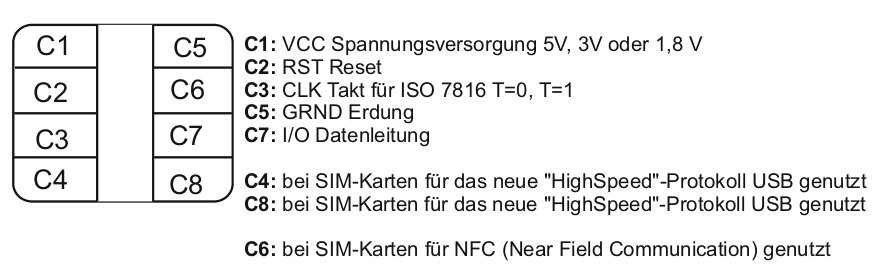
\includegraphics[width=410pt]{pinbelegung_chipkartensicherheit}
  \end{center}
  \caption[Pinbelegung einer Chipkarte]{Pinbelegung einer Chipkarte nach ISO/IEC 786 \cite{spitz11}}
  \label{abb:pinbelegung_chipkarten}
 \end{figure}

 \begin{figure}[htp]
  \begin{center}
   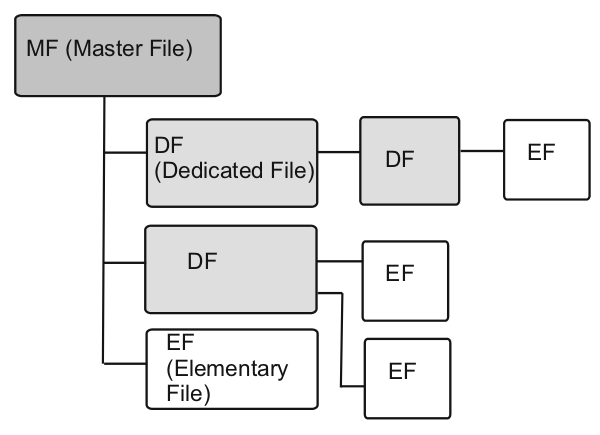
\includegraphics[width=350pt]{filesystem_chipkarten_chipkartensicherheit}
  \end{center}
  \caption[Filesystemarchitektur einer Chipkarte]{Filesystemarchitektur einer Chipkarte nach ISO/IEC 786 \cite{spitz11}}
  \label{abb:filesystem_chipkarten}
 \end{figure}

  \begin{figure}[htp]
  \begin{center}
   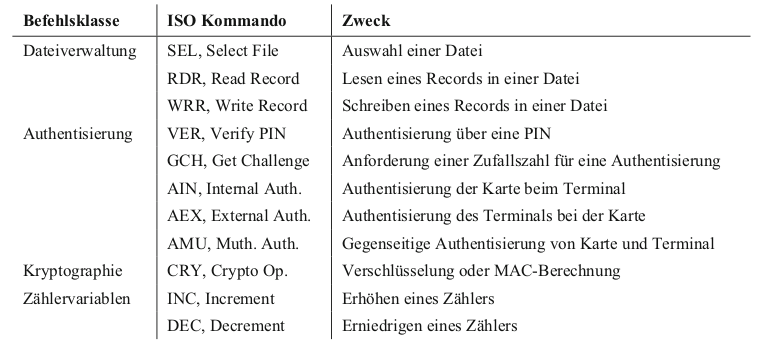
\includegraphics[width=460pt]{befehlsklassen_chipkartensicherheit}
  \end{center}
  \caption[Befehlsklassen einer Chipkarte]{Befehlsklassen einer Chipkarte nach ISO/IEC 786 \cite{spitz11}}
  \label{abb:befehlsklassen_chipkarten}
 \end{figure}

  \begin{figure}[htp]
  \begin{center}
   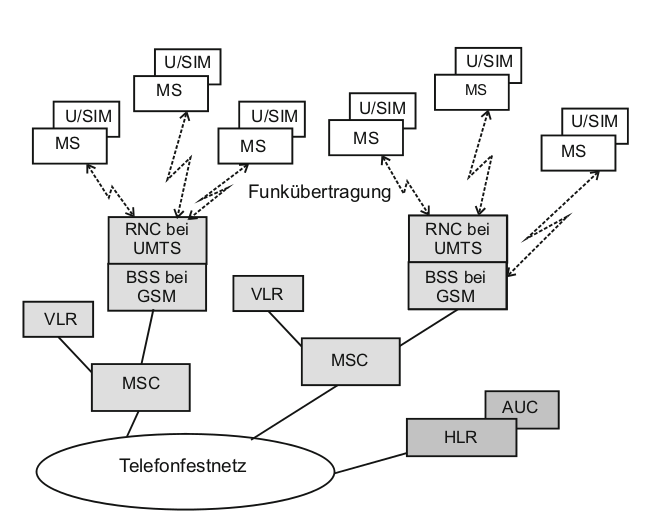
\includegraphics[width=380pt]{teilnehmer_telefonnetz_chipkartensicherheit}
  \end{center}
  \caption[Teilnehmer in Mobilfunknetzen]{Teilnehmer in Mobilfunknetzen (GSM und UMTS) \cite{spitz11}}
  \label{abb:teilnehmer_telefonnetz}
 \end{figure}

  \begin{figure}[htp]
  \begin{center}
   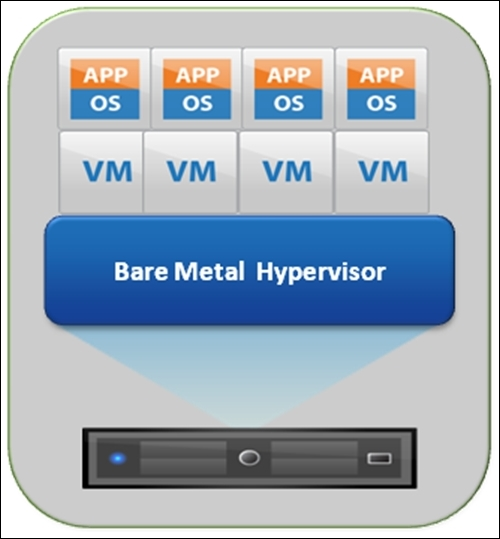
\includegraphics[width=200pt]{hypervisor_type1_dash13}
  \end{center}
  \caption[Architektur eines Typ-1-Hypervisors]{Architektur eines Typ-1-Hypervisors \cite{dash13}}
  \label{abb:hypervisor_type1}
 \end{figure}

  \begin{figure}[htp]
  \begin{center}
   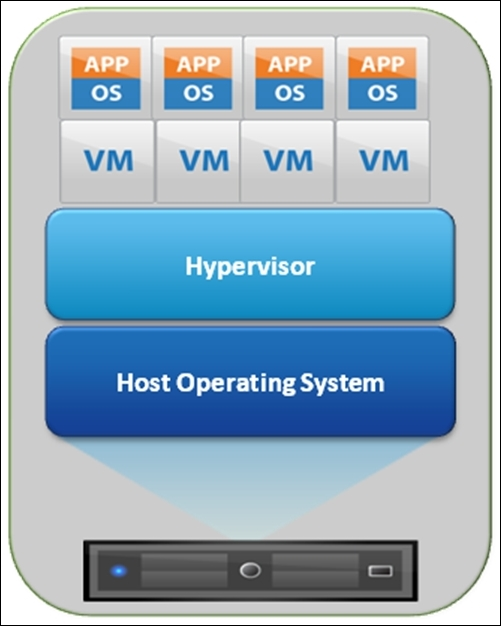
\includegraphics[width=200pt]{hypervisor_type2_dash13}
  \end{center}
  \caption[Architektur eines Typ-2-Hypervisors]{Architektur eines Typ-2-Hypervisors \cite{dash13}}
  \label{abb:hypervisor_type2}
 \end{figure}

  \begin{figure}[htp]
  \begin{center}
   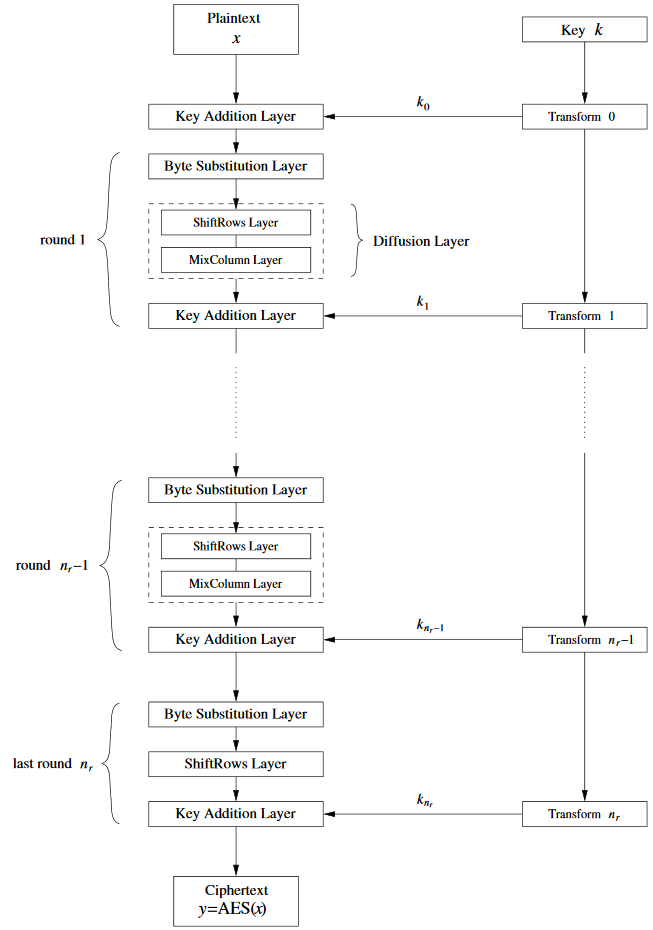
\includegraphics[width=440pt]{ablauf_aes}
  \end{center}
  \caption[Grafische Darstellung der AES-Verschlüsselung]{Grafische Darstellung der AES-Verschlüsselung \cite{paar10}}
  \label{abb:funktion_aes}
 \end{figure}
 
  \begin{figure}[htp]
  \begin{center}
   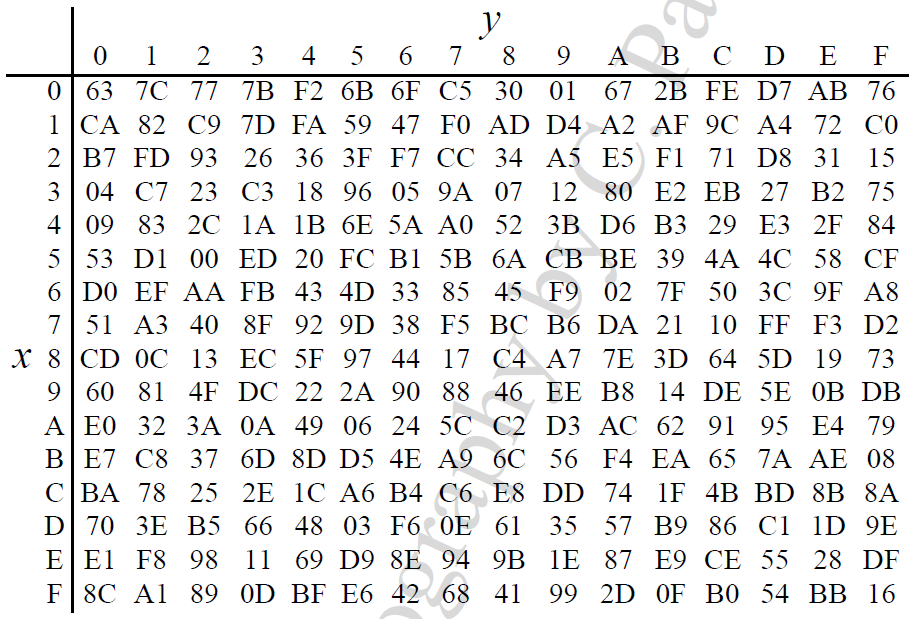
\includegraphics[width=440pt]{s-box}
  \end{center}
  \caption[Substitutionstabelle für AES-Verschlüsselung]{Substitutionstabelle für AES-Verschlüsselung \cite{paar10}}
  \label{abb:s-box}
 \end{figure}
 
 \begin{figure}[htp]
  \begin{center}
   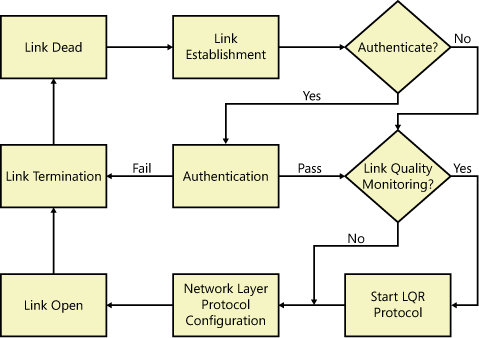
\includegraphics[width=350pt]{aufbauphasen_pppverbindung}
  \end{center}
  \caption[Aufbauphasen einer PPP-Verbindung]{Aufbauphasen einer PPP-Verbindung \cite{zackercomptia}}
  \label{abb:aufbauphasen_pppverbindung}
 \end{figure}

 \begin{figure}[htp]
  \begin{center}
   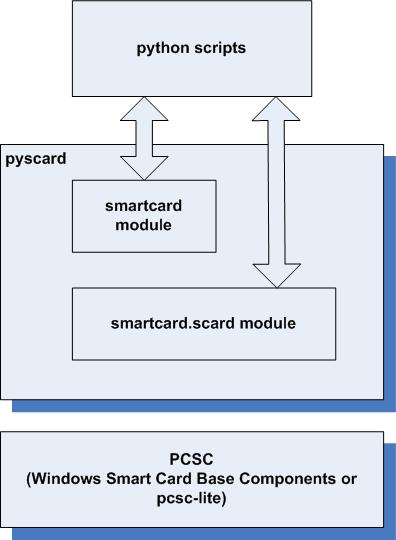
\includegraphics[width=350pt]{pyscard_schema}
  \end{center}
  \caption[Architektur der pyscard-Bibliothek]{Architektur der pyscard-Bibliothek \cite{pyscardweb}}
  \label{abb:pyscard_schema}
 \end{figure}

 \clearpage

\subsection{Listings}

  \lstinputlisting[caption=main.c, language=c, label=lst:main.c]{main.c}

  \lstinputlisting[caption=milenage.c, label=lst:milenage.c]{milenage.c}

  \lstinputlisting[caption=rijndael.c, language=c, label=lst:rijndael.c]{rijndael.c}

  \lstinputlisting[caption=client.py, language=python, label=lst:client.py]{client.py}

  \lstinputlisting[caption=..ppp/pppoe.conf, label=lst:pppoe.conf]{pppoe_conf}
 
% \lstinputlisting[caption=...ppp/allip, label=lst:allip]{allip}

 \lstinputlisting[caption=...ppp/pppoe-server-options, label=lst:pppoe_server_options]{pppoe-server-options}

 \lstinputlisting[caption=...init.d/pppoed, language=bash, label=lst:pppoe_init]{pppoed_init}

}

\pagestyle{empty}
%\section*{\reporttype}

%\begin{xlist}{xxxxxxxxxxxxxxxxxxxxxxxx} 
 % 		\item[\textbf{Titel}]        			\reporttitle
%		\item[\textbf{Subtitel}]          		\reportsubtitle
%		\item[\textbf{Autor}]          			\student
%		\item[\textbf{Hochschule}]          	\dhbw
%		\item[\textbf{Datum}]          			\handoverdate
%		\item[\textbf{Bearbeitungszeitraum}] 	\timerange
%		\item[\textbf{Studiengang}]          	\studiengang
%		\item[\textbf{Matrikelnummer, Kurs}]  	\matrikel, \kurs
%		\opt{PA}{
%			\item[\textbf{Ausbildungsfirma}]      	\company, \lokation
%		}
%		\opt{Bachelor}{
%			\item[\textbf{Ausbildungsfirma}]      	\company, \lokation
%		}
%		\item[\textbf{Betreuer}]   				\tutor
%		\item[\textbf{Gutachter}]            	\prof
%\end{xlist}
 	
\section*{Abstract}
\subsection*{Autoren}
\begin{addmargin}[1em]{2em}
Marco Heumann und Marco Schenkel
\end{addmargin}

\subsection*{Thema der Arbeit}
\begin{addmargin}[1em]{2em}
Programmierung einer SIM-Authentifizierung
\end{addmargin}

\subsection*{Stichworte}
\begin{addmargin}[1em]{2em}
Authentifizierung, SIM-Karten, UMTS
\end{addmargin}

\subsection*{Kurzzusammenfassung}
\begin{addmargin}[1em]{2em}
In dieser Arbeit wurde die Authentifizierung einer SIM-Karte
bei einem Netzprovider nachgebaut. Die Idee dahinter ist, dass
ein Hotel seinen Gästen eine SIM-Karte gibt. Diese müssen die
Karte in ihrem Zimmer in ein Kartenlesegerät stecken und bekommen
dann Zugang zum Internet. \\
In dieser Arbeit wird der UMTS Standard verwendet. Dieser benutzt
zur Authentifizierung den Milenage Algorithmus und damit verbunden
die standardisierte Blockchiffre AES.

Umgesetzt wurde in dieser Arbeit der Authentifizierungsvorgang. Dazu
wurde eine virtuelle Umgebung aufgesetzt in der die Authentifizierungsschnittstelle
läuft. Das Programm, welches in dieser Umgebung läuft und das die Berechnungen
des Milenage und AES Algorithmus durchführt, wurde in der Sprache C
geschrieben. \\
Auf der anderen Seite wurde ein Raspberry Pi verwendet, an dem ein Kartenlesegerät zum lesen der SIM-Karte
angeschlossen ist. Die SIM-Karte wird über den Linux-Treiber
PCSClite angesprochen. Ein Pythonprogramm steuert über den Treiber die Kommunikation
mit der SIM-Karte. \\
Die Kommunikation zwischen der virtuellen Umgebung und Raspberry Pi läuft über
ein Ethernetkabel und dem PPPoE-Protokoll.

Abschließend wird sowohl eine Auswertung über den Ablauf des Projektes als auch
eine Diskussion, welche mögliche Projekterweiterungen anspricht, ausgeführt.
\end{addmargin}

\clearpage

%\section*{\reporttype}

%\begin{xlist}{xxxxxxxxxxxxxxxxxxxxxxxxxx} 
%  		\item[\textbf{Title}]        			 	\reporttitle
%		\item[\textbf{Subtitle}]          		 	\reportsubtitle
%		\item[\textbf{Author}]          		 	\student
%		\item[\textbf{University}]          	 	\dhbw
%		\item[\textbf{Date}]          		 	   	\handoverdate
%		\item[\textbf{Time of Project}]             \timerange
%		\item[\textbf{Study Course}]          	 	\studiengang
%		\item[\textbf{Student ID, Course}]  		\matrikel, \kurs
%		\opt{PA}{
%			\item[\textbf{Company}]      			   	\company, \lokation
%		}
%		\opt{Bachelor}{
%			\item[\textbf{Company}]      			   	\company, \lokation
%		}
%		\item[\textbf{Supervisor in the Company}]   \tutor
%		\item[\textbf{Reviewer}]            		\prof
%\end{xlist}
 	
%\section*{Abstract}
%\lipsum[3-4] 

\end{document}
